\documentclass[a4paper]{article}

\usepackage[english]{babel}
\usepackage[utf8]{inputenc}
\usepackage{amsmath}
\usepackage{graphicx}
%\usepackage[colorinlistoftodos]{todonotes}
\usepackage{tikz}
\usetikzlibrary{arrows}
\usepackage{booktabs}
\usepackage{threeparttable}
\usepackage{tikz}
\usetikzlibrary{arrows.meta}
\usepackage{pgfplots}
\usepackage{subcaption}
\usepackage[toc,page]{appendix}
\usepackage{bm}
\usepackage{amsfonts}
\usepackage{algorithm,algpseudocode}
\usepackage{ulem}
\usepackage{footmisc}

\makeatletter
\newenvironment{breakablealgorithm}
{% \begin{breakablealgorithm}
	\begin{center}
		\refstepcounter{algorithm}% New algorithm
		\hrule height.8pt depth0pt \kern2pt% \@fs@pre for \@fs@ruled 
		\renewcommand{\caption}[2][\relax]{% Make a new \caption
			{\raggedright\textbf{\ALG@name~\thealgorithm} ##2\par}%
			\ifx\relax##1\relax % #1 is \relax
			\addcontentsline{loa}{algorithm}{\protect\numberline{\thealgorithm}##2}%
			\else % #1 is not \relax
			\addcontentsline{loa}{algorithm}{\protect\numberline{\thealgorithm}##1}%
			\fi
			\kern2pt\hrule\kern2pt
		}
	}{% \end{breakablealgorithm}
		\kern2pt\hrule\relax% \@fs@post for \@fs@ruled 
	\end{center}
}
\makeatother

\newcommand{\wt}{\widetilde}


\title{Fourth order summation-by-parts finite difference methods for  3-D elastic wave propagation in curvilinear coordinates with mesh refinement interfaces}

\date{\today}
\author{ Lu Zhang \and Siyang Wang \and N. Anders Petersson}
\begin{document}
\maketitle

\begin{abstract}
We analyze
\end{abstract}

%!TEX root = SISC_elastic_3d.tex
\section{Introduction}
Seismic wave propagation has important applications in earthquake simulation and forcasting, energy resources exploration, and underground motion analysis. In many practical problems, wave motion is governed by the three dimensional (3D) anisotropic elastic wave equations. The layered structure of the Earth gives rise to a piecewise smooth material property with discontinuities at internal interfaces, which are often curved in realistic models. Because of the heterogeneous material property and internal interfaces, the governing equations cannot be solved analytically, and it is necessary to use advanced numerical techniques to solve the seismic wave propagation problems.

When soving hyperbolic partial differential equations (PDEs), for computational efficiency, it is essential that the numerical methods are high order accurate (fourth order or higher). This is because high order methods have much smaller dispersion error than lower order methods, see the analysis of dispersion relation for first order hyperbolic PDEs \cite{Kreiss1972} and second order hyperbolic PDEs \cite{Hagstrom2012}. However, it is challenging to obtain high order accuracy in the presense of discontinuous material property and non-trivial geometry. 

Traditionally, the governing equations of seismic wave propagation are solved as a first order system, either in velocity-strain or velocity-stress formulation, which consists of nine equations. With the finite difference method, staggered grids are often used for first order systems, and recently the technique has been generalized to staggered curviliear grids for the wave equation \cite{OReilly2020}.

In this paper, we use another approach that discretizes the governing equations in second order form. Comparing with nine PDEs in a first order system, the second order formulation consists of only three PDEs in the displacement variables. In many cases, this could be a more effficient approach in terms of accuracy and memory usage. For spatial discretization, we consider the finite difference operators constructed in \cite{sjogreen2012fourth} that satisfy a summation-by-parts (SBP) principle. The SBP is a discrete analogue of the integration-by-parts, and is an important ingradient to obtain energy stability. 

In the SBP finite difference framework, a multi-block approach is often taken when the material property is discontinuous. That is, the domain is divided into subdomains such that the internal interfaces are aligned with the material discontinuities. SBP operators are then used independently in each subdomain for the spatial discretization of the governing equations. To patch subdomains together, physical interface conditions are imposed at internal interfaces. 


%There are two main methodologies to impose boundary and interface conditions in an SBP finite difference method. The  can be imposed weakly by using the simultaneous-approximation term (SAT) \cite{Carpenter1994}, which bears similarity with the discontinuous Galerkin method \cite{Gassner2013}. An SBP-SAT finite difference method has been developed to solve the elastic wave equation in \cite{Duru2014V}. Another approach is to impose boundary and interface conditions strongly by using ghost points, which is the approach taken in this paper. 

In \cite{petersson2015wave}, a fourth order SBP finite difference method is developed to solve the 3D elastic wave equation in heterogeneous smooth media, where topography in non-rectangular domains is resolved by using curvilinear meshes. The main objective of the present paper is to develop a fourth order method that solves the governing equations in piecewise smooth media, where material discontinuities occur at curved interfaces. This is motivated by the fact that in realistic models, material properties are only piecewise smooth with discontinuities, and it is important to obtain high order accuracy even at the material interfaces. A highlight of our method is that  mesh sizes in each subdomain can be chosen according to the velocity structure of the material property so that computational efficiency is maximized. In the context of seismic wave propagation, as going deeper in the Earth, the wave speed gets larger and the wavelength gets longer. Correspondingly, in our model, the mesh becomes coarser from one subdomain to the next one underneath. In this way, the number of grid points per wavelength can be kept almost the same in the entire domain. 

For mesh refinement interfaces, we have constructed fourth order interpolation and restriction operators to impose the interface conditions at the hanging nodes. These operators are compatible with the underlying SBP operators. With a fourth order predictor-corrector time integrator, the fully discrete discretization is energy conserving. 

The rest of the paper is organized as follows. In Sec. 2, we introduce the governing equations in curvilinear coordinates. The spatial discretization is presented in detail in Sec. 3. Particular emphasize is placed on the numerical coupling procedure at curved mesh refinement interfaces. In Sec. 4, we describe the temporal discretization, and present the fully discrete scheme. Numerical experiments are presented in Sec. 5 to verify the convergence rate of the proposed scheme and the energy conserving property. We also demonstrate that the mesh refinement interfaces do not introduce spurious wave reflections. In the end, we draw conclusion in Sec. 6. 


%!TEX root = elastic_3d_sbp.tex
\section{The isotropic elastic wave equation }
We consider the time dependent isotropic elastic wave equation in three dimensional domain for simple Cartesian domain and the curvilinear domian.

%!TEX root = elastic_3d_sbp.tex
\subsection{The Cartesian coordinates}
The problem is defined on the domain ${\bf x}\in\Omega = [0,a^{(1)}]\times[0,a^{(2)}]\times[0,a^{(3)}]$ with ${\bf x} = (x^{(1)},x^{(2)},x^{(3)})^T$ are Cartesian coordinates. Denote ${\bf u} = (u_1,u_2,u_3)^T$ to be the three dimensional displacement vector in Cartesian coordinates, then the elastic wave equation takes the form,
\begin{align*}
\rho\frac{\partial^2{\bf u}}{\partial^2 t} &= \nabla\cdot\mathcal{T} + {\bf F}, \ \ \ {\bf x}\in\Omega,\ \ \ t\geq 0,\\
\nabla\cdot\mathcal{T} &:= L{\bf u},
\end{align*}
provided with appropriate initial and boundary conditions, especially, we consider periodic boundary conditions in the directions $1$ and $2$ for the rest of the paper and the boundary conditions in the direction $3$ will be given later. Here, $\rho$ is density, $\mathcal{T}$ is the stress tensor and ${\bf F}$ is the force function. The spatial operator $L$ is called $3\times3$ symmetric Kelvin-Christoffel differential operator matrix, specifically,
\begin{equation*}
L{\bf  u} = \partial_1(A_1\nabla{\bf u}) + \partial_2(A_2\nabla{\bf u}) + \partial_3(A_3\nabla{\bf u}),
\end{equation*}
with
\begin{align*}
A_1\nabla{\bf u} &:= M_{11}\partial_1{\bf u} + M_{12}\partial_2{\bf u} + M_{13}\partial_3{\bf u}, \\
A_2\nabla{\bf u} &:= M_{21}\partial_1{\bf u} + M_{22}\partial_2{\bf u} + M_{23}\partial_3{\bf u}, \\
A_3\nabla{\bf u} &:= M_{31}\partial_1{\bf u} + M_{32}\partial_2{\bf u} + M_{33}\partial_3{\bf u},
\end{align*}
where $M_{ij}, i,j = 1,2,3$ are defined by
\begin{equation}\label{Mmatrices}
M_{ij} = P^T_iCP_j.
\end{equation}
Here, $C$ is symmetric and positive definite, we refer to Appendix ? for the definitions of matrices $C$ and $P_i, i = 1,2,3$. For the matrices $M_{ij}$, we have that $M_{ii}$ are symmetric positive definite, and $M_{ij}=M^T_{ji}$, for $i,j=1,2,3$. Especially, for the isotropic elastic wave equation, we have
\[ M_{11} = \left(\begin{array}{ccc}
2\mu+\lambda & 0 & 0\\
0 & \mu & 0\\
0 & 0 & \mu\end{array}\right), M_{12} = \left(\begin{array}{ccc}
0 & \lambda & 0\\
\mu & 0 & 0\\
0 & 0 & 0\end{array}\right), M_{13} = \left(\begin{array}{ccc}
0 & 0 & \lambda\\
0 & 0 & 0\\
\mu & 0 & 0\end{array}\right),\]
\[ M_{21} =(M_{12})^T, M_{22} = \left(\begin{array}{ccc}
\mu & 0 & 0\\
0 & 2\mu+\lambda & 0\\
0 & 0 & \mu\end{array}\right), M_{23} = \left(\begin{array}{ccc}
0 & 0 & 0\\
0 & 0 & \lambda\\
0 & \mu & 0\end{array}\right),\]
\[ M_{31} = (M_{13})^T, \ \ \ \ \ M_{32} =(M_{23})^T, \ \ \ \ \ M_{33} = \left(\begin{array}{ccc}
\mu & 0 & \lambda\\
0 & \mu & 0\\
0 & 0 & 2\mu+\lambda\end{array}\right),\]
Here, $\lambda$ and $\mu$ are the first and second Lame parameters respectively, which are determined by the properties of the materials.

Denote the unit outward normal ${\bf n}_i^{\pm} = (n_i^{\pm,(1)},n_i^{\pm,(2)},n_i^{\pm,(3)})$ for the boundaries $x^{(i)} = 0, a^{(i)}, i = 1,2,3$ respectively. For example, ${\bf n}_1^{\pm} = (\pm 1, 0,0)$ for the boundaries $x^{(1)} = a^{(1)}$ and $x^{(1)} = 0$ respectively, then we have the boundary traction forcing 
\begin{equation*}
{\bf n}_i^{\pm}\cdot\mathcal{T} = n^{\pm,(1)}_iA_1\nabla{\bf u} + n^{\pm,(2)}_iA_2\nabla{\bf u} + n^{\pm,(3)}_iA_3\nabla{\bf u},\ \ i = 1,2,3.
\end{equation*}
A homogeneous Dirichlet boundary condition corresponds to ${\bf u} = {\bf 0}$ and a free surface boundary condtion is ${\bf n}_i^{\pm}\cdot\mathcal{T}  = {\bf 0}, i = 1,2,3$.

It is known that the elastic wave equation with the homogeneous Dirichelet boundary conidtion or free surface boundary condition in a Cartesian domain is a well-posed problem and the total energy of the solution is conserved if the external force ${\bf F} = 0$, we refer to \cite{?} for a detailed analysis.


%!TEX root = elastic_3d_sbp.tex
\subsection{Generalization to curvilinear coordinates}
%Present the transformed equation. Notation is important. We can write a few formulas first, and discuss if it is good notation. Maybe we shall follow notations from one of Anders' papers?

In this section, we consider a curvilinear domain $\Omega$. Assume there is a one-to-one mapping ${\bf x} = {\bf x}({\bf r}) : [0,1]^3 \rightarrow \Omega \subset \mathbb{R}^3$ with ${\bf x}({\bf r}) = (x^{(1)}({\bf r}),x^{(2)}({\bf r}),x^{(3)}({\bf r}))^T, {\bf r} = (r^{(1)},r^{(2)},r^{(3)})^T, 0\leq r^{(i)}\leq1, i = 1,2,3$. We define the derivative of the forward mapping to be 
\begin{equation}\label{elastic_eq_carte}
{\bf a}_k := \bar{\partial}_k{\bf x} = \left(\frac{\partial x^{(1)}}{\partial r^{(k)}},\frac{\partial x^{(2)}}{\partial r^{(k)}},\frac{\partial x^{(3)}}{\partial r^{(k)}}\right)^T,
\end{equation}
for $k = 1,2,3$ and the backward mapping to be
\begin{equation*}
{\bf a}^k := \nabla r^{(k)} = \left(\frac{\partial r^{(k)}}{\partial x^{(1)}},\frac{\partial r^{(k)}}{\partial x^{(2)}},\frac{\partial r^{(k)}}{\partial x^{(3)}}\right)^T := (\xi_{1k},\xi_{2k},\xi_{3k})^T,
\end{equation*}
for $k = 1,2,3$. It is known that the backward mapping can be expressed by the forward mapping \cite{?}, 
\begin{equation*}
{\bf a}^i = \frac{1}{J}({\bf a}_j\times{\bf a}_k), \ \ \ (i,j,k) \ \text{cycle}.
\end{equation*}
Here, $J:=\text{det}({\bf a}_1, {\bf a}_2, {\bf a}_3)$ is the Jacobian of the forward mapping. We assume that the mapping is non-singular such that  $0<J<\infty$.

After applying the forward and backward mapping, reader can refer to \cite{?} for details, the elastic wave equation (\ref{elastic_eq_carte}) can be written as
\begin{equation}\label{elastic_eq_curvi}
\rho\frac{\partial^2 {\bf u}}{\partial t^2} = \frac{1}{J}\left[\bar{\partial }_1(\bar{A}_1\bar{\nabla}{\bf u}) + \bar{\partial }_2(\bar{A}_2\bar{\nabla}{\bf u}) +\bar{\partial }_3(\bar{A}_3\bar{\nabla}{\bf u}) \right] + {\bf F},
\end{equation}
where
\begin{align*}
\bar{A}_1\bar{\nabla}{\bf u} &:= N_{11}\bar{\partial}_1{\bf u} + N_{12}\bar{\partial}_2{\bf u} + N_{13}\bar{\partial}_3{\bf u}, \\
\bar{A}_2\bar{\nabla}{\bf u} &:= N_{21}\bar{\partial}_1{\bf u} + N_{22}\bar{\partial}_2{\bf u} + N_{23}\bar{\partial}_3{\bf u}, \\
\bar{A}_3\bar{\nabla}{\bf u} &:= N_{31}\bar{\partial}_1{\bf u} + N_{32}\bar{\partial}_2{\bf u} + N_{33}\bar{\partial}_3{\bf u},
\end{align*}
here, 
\begin{equation}\label{definition_Nij}
N_{ij} = J\bar{P}_i^TC\bar{P}_j \ \ \text{with} \ \ \bar{P}_i = \sum_{j=1}^3\xi_{ji}P_j.
\end{equation}
The definitions of matrices $C$ and $P_i, i = 1,2,3$ can be found in Appendix ?. The matrices $N_{ij}$ have similar properties as the corresponding matrices $M_{ij}$ in the Cartesian case \eqref{Mmatrices}, that is $N_{ii}$ are symmetric positive definite, and $N_{ij}=N_{ji}^T$ for $i,j=1,2,3$ with $i\ne j$.

The transformation of Dirichlet boundary condition between parameter coordinates and curvilinear coordinates is straightfroward, ${\bf u}({\bf x}) = {\bf u}(\bf r)$. To transfer the boundary forcing condition from curvilinear coordinates to parameter coordinates, we firstly write the unit outside normal to be the function of metric derivatives, for example, along the boundary $r^{(3)} = 1$ or $r^{(3)} = 0$,
\begin{equation}\label{definition_bdry3_curvi}
{\bf n}_3^{\pm} := (n^{\pm,(1)}_3,n^{\pm,(2)}_3,n^{\pm,(3)}_3)^T = \pm \frac{\nabla r^{(3)}}{\left|\nabla r^{(3)}\right|} = \frac{\pm 1}{\sqrt{((\xi_{13})^2+(\xi_{23})^2+(\xi_{33})^2)}}\left(\xi_{13},\xi_{23},\xi_{33}\right)^T,
\end{equation}
here, $'+'$ corresponds to $r^{(3)} = 1$ and $'-'$ corresponds to $r^{(3)} = 0$. Then after some straightforward calculations, the boundary forcing condition can be written as
\begin{equation}\label{bdry3_curvi}
\mathcal{T}\cdot{\bf n}_3^{\pm} = \frac{\pm 1}{J\left|\nabla r^{(3)}\right|}\bar{A}_3\bar{\nabla}{\bf u}, \ \ \ r^{(3)} = 1, 0.
\end{equation}
Similarly, we can derive the boundary forcing condition along $r^{(1)} = 0,1$ and $r^{(2)} = 0,1$ as
\begin{equation}\label{bdry1_curvi}
\mathcal{T}\cdot{\bf n}_1^{\pm} = \frac{\pm 1}{J\left|\nabla r^{(1)}\right|}\bar{A}_1\bar{\nabla}{\bf u}, \ \ \ r^{(1)} = 1, 0,
\end{equation}
\begin{equation}\label{bdry2_curvi}
\mathcal{T}\cdot{\bf n}_2^{\pm} = \frac{\pm 1}{J\left|\nabla r^{(2)}\right|}\bar{A}_2\bar{\nabla}{\bf u}, \ \ \ r^{(2)} = 1, 0,
\end{equation} 
respectively. Here, the ${\bf n}_1^{\pm}$ and ${\bf n}_2^{\pm}$ have a similar definition as ${\bf n}_3^{\pm}$ in (\ref{definition_bdry3_curvi}).


%!TEX root = SISC_elastic_3d.tex
\subsection{Energy estimate}\label{sec_energy}
In this section, we derive an energy estimate for the semi-discretization (\ref{elastic_semi_c}) and (\ref{fine_scheme}) in Sec.~\ref{semi_discrete_form}. Let ${\bf u}, {\bf v}$ be grid functions in the coarse domain $\Omega^c$ and define the three dimensional discrete scalar product in $\Omega^c$ as
\begin{equation}\label{scalar_product_inner}
({\bf v}, {\bf u})_{2h} = 8h_1h_2h_3\sum_{i=1}^{n_1^{2h}}\sum_{j=1}^{n_2^{2h}}\sum_{k=1}^{n_3^{2h}}\omega_k{J}_{i,j,k}^{c}({\bf v}_{i,j,k}\cdot {\bf u}_{i,j,k}).
\end{equation}
Similarly, define the three dimensional discrete scalar product in $\Omega^f$ as
\begin{equation}\label{scalar_product_inner_f}
({\bf v}, {\bf u})_{h} = h_1h_2h_3\sum_{i=1}^{n_1^{h}}\sum_{j=1}^{n_2^{h}}\sum_{k=1}^{n_3^{h}}\omega_k{J}_{i,j,k}^{f}({\bf v}_{i,j,k}\cdot {\bf u}_{i,j,k}),
\end{equation}
where $\bf u$ and $\bf v$ are grid functions in the fine domain $\Omega^f$. Now, we are ready to state the energy estimate of the proposed schemes in Section \ref{semi_discrete_form}. 
\begin{theorem}\label{thm1}
	The semi-discretization (\ref{elastic_semi_c}) and (\ref{fine_scheme}) is energy stable if the interface conditions \eqref{continuous_sol} and \eqref{continuous_traction} are satisfied.
\end{theorem}
\begin{proof}
	%Let $\rho^{h}, \rho^{2h}$ be diagonal matrices. Their diagonal elements are $\rho^f, \rho^c$ evaluated at grid points in $\Omega^f$ and $\Omega^c$, respectively; let $J^{h}, J^{2h}$ be diagonal matrices. Their diagonal elements are $J^f, J^c$ evaluated at grid points in $\Omega^f$ and $\Omega^c$, respectively.
		Let $\rho^{h}$, $\rho^{2h}$, $J^{h}$ and $J^{2h}$ be diagonal matrices with diagonal elements equal to the corresponding continuous functions evaluated on the grid, respectively. 
	By forming the inner product between (\ref{elastic_semi_c}) and $8h_1h_2h_3\omega_k(J^{2h}\otimes {\bf I}){\bf c}_t$, based on \eqref{scalar_product_inner}, we have
	\begin{equation}\label{coarse_simple}
	({\bf c}_t, (\rho^{2h}\otimes {\bf I}){\bf c}_{tt})_{2h} = ({\bf c}_t,(J^{2h}\otimes {\bf I})^{-1}\wt{\mathcal{L}}^{2h}{\bf c})_{2h} = -\mathcal{S}_{2h}({\bf c}_t,{\bf c}) + B_{2h}({\bf c}_t,{{\bf c}}),
	\end{equation}
	where $\mathcal{S}_{2h}({\bf c}_t,{\bf c})$ is a symmetric and positive definite bilinear form given in Appendix \ref{appendix_bf}, the boundary term $B_{2h} ({\bf c}_t,{\bf c})$ is given by
	\begin{equation}\label{bounary_c1}
	B_{2h} ({\bf c}_t,{\bf c}) = 4h_1h_2\sum_{{\bf i}\in I_{\Gamma^c}}\frac{d{\bf c}_{\bf i}}{dt}\cdot (\wt{A}_3^{2h}{\bf c}_{\bf i}).
	\end{equation}
	By forming the inner product between (\ref{fine_scheme}) and $h_1h_2h_3\omega_k(J^h\otimes {\bf I}){\bf f}_t$, based on \eqref{scalar_product_inner_f}, we obtain
	\begin{equation}\label{fine_simple}
	({\bf f}_t, (\rho^h\otimes {\bf I}){\bf f}_{tt})_h = ({\bf f}_t,(J^h\otimes {\bf I})^{-1}\hat{\mathcal{L}}^h{\bf f})_h = -\mathcal{S}_{h}({\bf f}_t,{\bf f}) + B_h({\bf f}_t,{\bf f}) 
	+h_1h_2h_3\omega_1\sum_{i = 1}^{n_1^h}\sum_{j=1}^{n_2^h} \frac{d{\bf f}_{i,j,1}}{dt}\cdot{\bm \eta}_{i,j,1}.
	\end{equation}
Here, $\mathcal{S}_h$ is also a symmetric and positive definite bilinear form given in Appendix \ref{appendix_bf}. The boundary term $B_h ({\bf f}_t,{\bf f})$ has the following form
	\begin{equation}\label{boundary_f1}
	B_h ({\bf f}_t,{\bf f}) = -h_1h_2\sum_{{\bf i}\in I_{\Gamma^f}}\frac{d{\bf f}_{\bf i}}{dt}\cdot(A_3^h {\bf f}_{\bf i}).
	\end{equation}
	 Adding \eqref{coarse_simple} and \eqref{fine_simple} together, we have
	\begin{multline}\label{semi_energy_1}
	\frac{d}{dt}\big[({\bf f}_t,(\rho^h\otimes {\bf I}) {\bf f}_t)_h + \mathcal{S}_{h}({\bf f},{\bf f}) + ({\bf c}_t,(\rho^{2h}\otimes {\bf I}) {\bf c}_t)_{2h} + \mathcal{S}_{2h}({\bf c},{\bf c}) \big]  = \\
	2B_{h}({\bf f}_t,{\bf f}) + 2B_{2h}({\bf c}_t,{\bf c}) + 2h_1h_2h_3\omega_1\sum_{i = 1}^{n_1^h}\sum_{j=1}^{n_2^h}\frac{d{\bf f}_{i,j,1}}{dt}\cdot{\bm \eta}_{i,j,1}.
	\end{multline}
	Substituting (\ref{boundary_f1}) and (\ref{bounary_c1}) into (\ref{semi_energy_1}) and combining the definitions of the scalar product at the interface (\ref{scalar_product_discrete_interface_c})--(\ref{scalar_product_discrete_interface_f}), the continuity of solution at the interface \eqref{continuous_sol} and Lemma \ref{lemma1}, we get
	\begin{align*}\label{semi_energy_2}
	&\hspace{0.4cm}\frac{d}{dt}\left[({\bf f}_t,(\rho^h\otimes {\bf I}) {\bf f}_t)_{h} + \mathcal{S}_{h}({\bf f},{\bf f}) + ({\bf c}_t,(\rho^{2h}\otimes {\bf I}) {\bf c}_t)_{2h} + \mathcal{S}_{2h}({\bf c},{\bf c}) \right]   \nonumber\\
	& = 2\left<{\bf f}_t,\big(({\Lambda}^{h}{J}^h_\Gamma\big)\otimes {\bf I})^{-1}(-\mathcal{A}_3^h{\bf f}+h_3\omega_1{\bm \eta})\right>_{h}+ 2\left<{\bf c}_t,\big(({\Lambda}^{2h}{J}^{2h}_\Gamma\big)\otimes{\bf I})^{-1}\wt{\mathcal{A}}_3^{2h}{\bf c}\right>_{2h} \nonumber\\
	& = 2\left<{\mathcal{P}}{\bf c}_t,\big(({\Lambda}^{h}{J}^h_\Gamma)\otimes{\bf I}\big)^{-1}(-\mathcal{A}_3^h{\bf f}+h_3\omega_1{\bm \eta})\right>_{h}+ 2\left<{\bf c}_t, \big(({\Lambda}^{2h}{J}^{2h}_\Gamma)\otimes{\bf I}\big)^{-1}\wt{\mathcal{A}}_3^{2h}{\bf c}\right>_{2h} \nonumber\\
	& = 2\left<{\bf c}_t,{\mathcal{R}}\Big(\big(({\Lambda}^{h}{J}^h_\Gamma)\otimes{\bf I}\big)^{-1}(-\mathcal{A}_3^h{\bf f}+h_3\omega_1{\bm \eta})\Big)\right>_{2h}+ 2\left<{\bf c}_t,\big(({\Lambda}^{2h}{J}^{2h}_\Gamma)\otimes{\bf I}\big)^{-1}\wt{\mathcal{A}}_3^{2h}{\bf c}\right>_{2h} = 0.
	\end{align*}
Note that the discrete energy for the semi-discretization \eqref{elastic_semi_c} and \eqref{fine_scheme} is given by $({\bf f}_t,(\rho^h\otimes {\bf I}) {\bf f}_t)_{h} + \mathcal{S}_{h}({\bf f},{\bf f}) + ({\bf c}_t,(\rho^{2h} \otimes {\bf I}){\bf c}_t)_{2h} + \mathcal{S}_{2h}({\bf c},{\bf c})$.
\end{proof}








 

%!TEX root = SISC_elastic_3d.tex
\section{The spatial discretization}

In this section, we describe the spatial discretization for the problem (\ref{elastic_curvi}). We firstly introduce the SBP operator for the first and second spatial derivative with a scalar variable in one dimension and then extend the SBP operators to vector variables in three dimensions.

%!TEX root = elastic_3d_sbp.tex
\subsection{SBP operators in $1$D}\label{sec_sbp_1d}
Consider a uniform discretization of the domain $x\in[0,1]$ with the grids,
\[\uline{\wt
	{{\bf x}}} = [x_0,x_1,\cdots,x_n,x_{n+1}]^T,\ \  x_i = (i-1)h,\ \ i = 0,1,\cdots,n,n+1,\ \ h = 1/(n-1),\]
where $i = 1,n$ correspond to the grid points on the boundary, and $i = 0,n+1$ are ghost points outside the physical domain.
We also denote ${\bf x} = [x_1,x_2,\cdots,x_n]^T$ the grids that does not  contain the ghost points, $\wt{{\bf x}} = [x_1,x_2,\cdots,x_n,x_{n+1}]^T$ the grids only conatin the ghost point on the right, $\uline{{\bf x}} = [x_0,x_1,x_2,\cdots,x_n]^T$ the grids only conatin the ghost point on the left. The  operator $D \approx \frac{\partial }{\partial x}$ is a first derivative SBP operator if 
\begin{equation}\label{first_sbp}
({\bf u}, D{\bf v})_h = -(D{\bf u},{\bf v})_h - u_1v_1 + u_nv_n,
\end{equation}
with a scalar product
\begin{equation}\label{inner_product}
({\bf u},{\bf v})_h = h\sum_{i = 1}^{n}\omega_iu_iv_i.
\end{equation}
Here, $0<\omega_i < \infty $ are the weights of scalar product. The SBP operator $D$ has a centered difference stencil at the grid points away from the boudnary and the corresponding weights $\omega_i = 1$. To satisfy the SBP identity (\ref{first_sbp}), the coefficients in $D$ are  modified at a few points near the boundary and the corresponding weights $\omega_i \neq 1$. The operator $D$ does not use any ghost points. 

To discretize the elastic wave equation, we also need to approximate the second derivative with variable coefficient $(\gamma(x)u_x)_x$. Here, the known function $\gamma(x)>0$ describes the property of the material. There are two different fourth order accurate SBP operators for the approximation of $(\gamma(x)u_x)_x$. The first one $\uline{\wt{G}}(\gamma){\bf u} \approx (\gamma(x)u_x)_x $, derived by Sj\"ogreen and Petersson \cite{?}, uses one ghost point outside each boundary, and satisfies the second derivative SBP identity,
\begin{equation}\label{sbp_2nd_1}
({\bf u}, \uline{\wt{G}}(\gamma){\bf v})_h = -S_\gamma({\bf u},{\bf v})-u_1\gamma_1\uline{\bf b}_1{\bf v} + u_n\gamma_n\wt{\bf b}_n {\bf v}.
\end{equation}
Here, the bilinear form $S_\gamma(\cdot,\cdot)$ is symmetric and positive semi-definite, and does not use any ghost points. The operators $\uline{\bf b}_1$ and $\wt{\bf b}_n$ aprroximate the first derivative on the left and right boundaries, respectively. Using the left boundary as an example, we have 
\begin{equation}\label{sbp_1st_1}
\wt{\bf b}_1 {\bf v} = \frac{1}{h}\sum_{i=0}^{4} \wt{d}_i v_i,
\end{equation}
as the fourth order accurate approximation of $u_x(x_1)$. We note that the notation $\uline{\wt{G}}(\gamma){\bf v}$ implies that the operator $\uline{\wt{G}}$ uses ${\bf v}$ on all grid points $\uline{\wt{{\bf x}}}$, but $\uline{\wt{G}}(\gamma){\bf v}$ only returns values on the grid ${\bf x}$ without ghost points. Therefore, when writing in matrix form, $\uline{\wt{G}}$ is a non-square matrix of size $n$ by $n+2$.

The other SBP operator ${G}(\gamma){\bf u} \approx (\gamma(x)u_x)_x $ is developed by Mattsson \cite{?} without using any ghost points, and satisfies a similar SBP identity,
\begin{equation}\label{sbp_2nd_2}
({\bf u}, G(\gamma){\bf v})_h = -S_\gamma({\bf u},{\bf v})-u_1\gamma_1{\bf b}_1{\bf v} + u_n\gamma_n{\bf b}_n{\bf v}.
\end{equation}
Here, ${\bf b}_1$ and ${\bf b}_n$ are also finite difference operators for the first derivative at the boundaries, but are constructed to third order accurate,
\begin{equation}\label{sbp_1st_2}
{\bf b}_1 {\bf v} = \frac{1}{h}\sum_{i=1}^{4} d_i v_i. 
\end{equation}
In this case, ${G}(\gamma)$ is square in matrix form. 

For the second derivative SBP operators $\uline{\wt{G}}(\gamma)$ and $G(\gamma)$, both of them use a fourth order five points centered difference stencil to approximate $(\gamma u_x)_x$ on the interior points away from the boundaries. For the first and the last six grid points close to the boudaries, the operators $G(\gamma)$ and $\uline{\wt{G}}(\gamma)$ use second order accurate one-sided difference stencils. They are designed to satisfy (\ref{sbp_2nd_2}) and (\ref{sbp_2nd_1}), respectively.  Note that we can derive two new second derivative SBP operators $\wt{G}(\gamma), \uline{G}(\gamma)$ based on $\uline{\wt{G}}(\gamma), G(\gamma)$ and they satisfy
\begin{equation}\label{sbp_2nd_3}
({\bf u}, \wt{G}(\gamma){\bf v})_h = -S_\gamma({\bf u},{\bf v})-u_1\gamma_1{\bf b}_1{\bf v} + u_n\gamma_n\wt{{\bf b}}_n{\bf v},
\end{equation}
and
\begin{equation}\label{sbp_2nd_4}
({\bf u}, \uline{G}(\gamma){\bf v})_h = -S_\gamma({\bf u},{\bf v})-u_1\gamma_1\uline{{\bf b}}_1{\bf v} + u_n\gamma_n{\bf b}_n{\bf v},
\end{equation}
respectively. Besides, in the matrix form, both of them are of size $n$ by $n+1$. In the following sections, we use all of them to develop a multi-block finite difference discretization for the elastic wave equation. 


%!TEX root = SISC_elastic_3d.tex
\subsection{Semi-discretization of the elastic wave equation}\label{semi_discrete_form}

\begin{figure}[htbp]
	\centering
	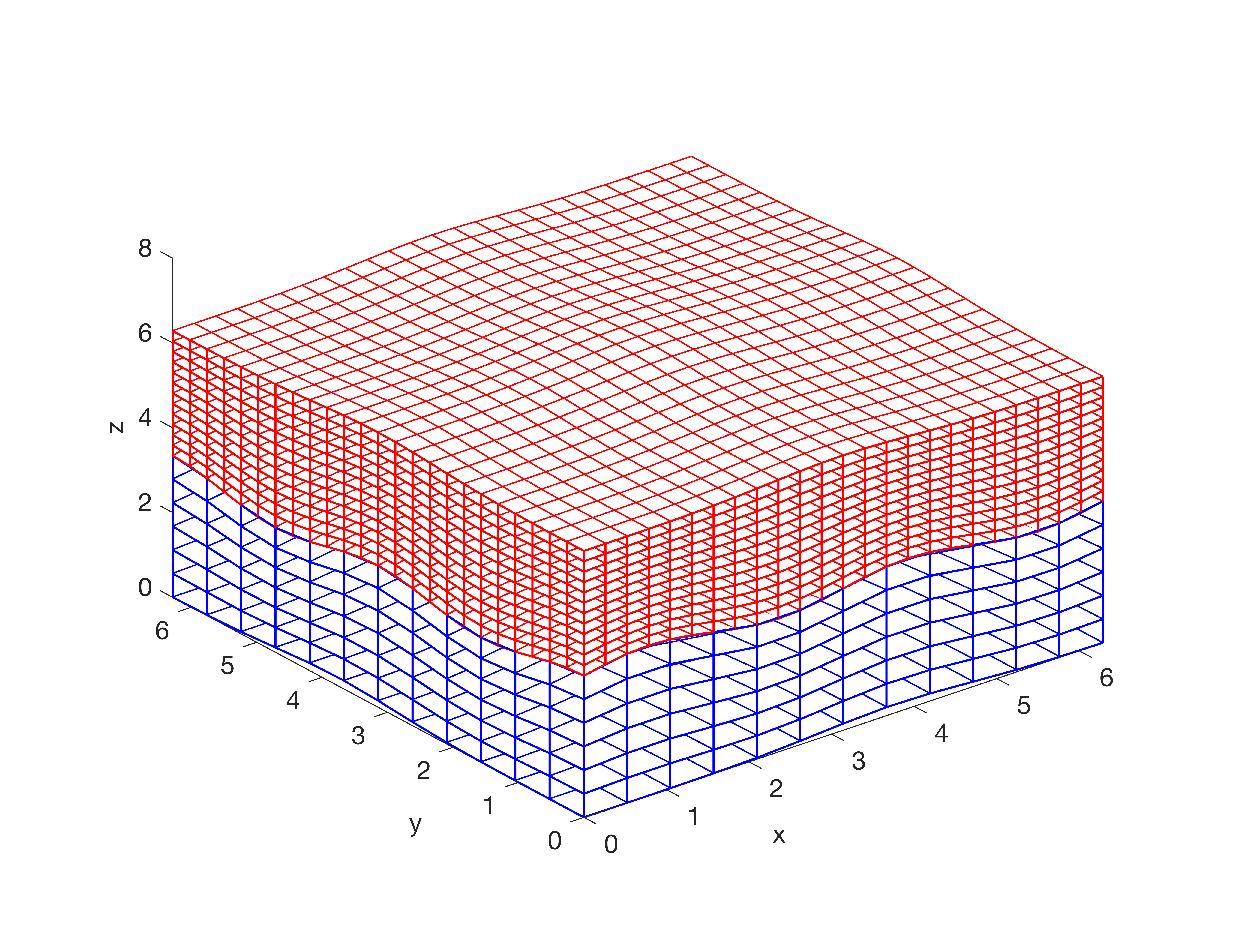
\includegraphics[width=0.6\textwidth,trim={0.4cm 0.7cm 0.8cm 1.4cm}, clip]{physical_discretization.eps}
	\caption{The sketch for the curvilinear mesh of the physical domain $\Omega$. The blue region is the spatial discretization of coarse subdomain $\Omega^c$ and the red region is the spatial discretization of the fine domain $\Omega^f$. Note that $x,y,z$ in the graph correspond to $x^{(1)}, x^{(2)}, x^{(3)}$ respectively. 
	 }\label{physical_discretization}
\end{figure}

In this section, we discretize the elastic wave equations (\ref{elastic_curvi}) and  (\ref{elastic_curvi_f}) with mesh refinement interface $\Gamma$. We assume the ratio of mesh sizes in the reference domains is $1:2$, that is the mesh sizes satisfy
\[h_1(n_1^h-1) = 1, \ \ \ h_2(n_2^h-1) = 1, \ \ \ h_3(n_3^h-1) = 1,\]
and
\[2h_1(n_1^{2h}-1) = 1, \ \ \ 2h_2(n_2^{2h}-1) = 1, \ \ \ 2h_3(n_3^{2h}-1) = 1,\]
respectively. Other ratios can be treated analogously. Figure \ref{physical_discretization} gives an illustration of the discretization of a physical domain. This is an ideal mesh if the wave speed in $\Omega^f$ is half of the wave speed in $\Omega^c$.

In seismic wave simulation, far-field boundary conditions are often imposed in the $x^{(1)}$ and $x^{(2)}$ directions. Here, our focus is on the numerical treatment of the interface conditions (\ref{interface_cond}). We assume periodic boundary conditions in $x^{(1)}$ and $x^{(2)}$, and ignore the boundaries in $x^{(3)}$. In Figure \ref{section_discretization}, we fix $x^{(2)} = 0$ and present the $x^{(1)}$-$x^{(3)}$ section of the domain $\Omega$ in both curvilinear space and parameter space.
\begin{figure}[htbp]
	\centering
	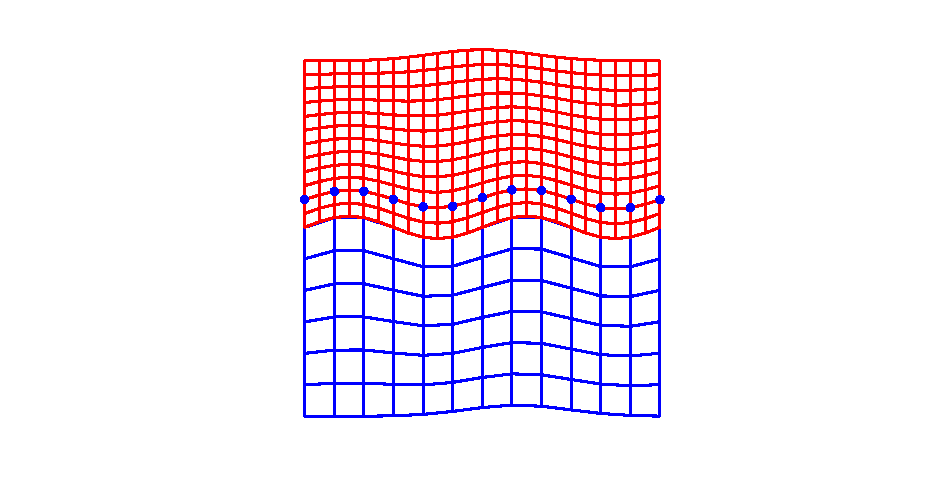
\includegraphics[width=0.45\textwidth,trim={1.0cm 2.0cm 1.0cm 1.8cm}, clip]{physical_section_discretization.eps}
	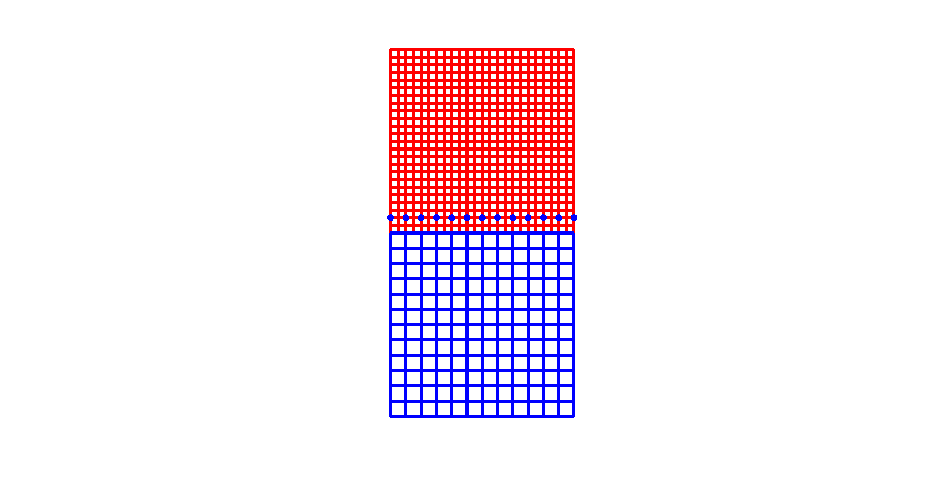
\includegraphics[width=0.45\textwidth,trim={1.0cm 2.0cm 1cm 1.8cm}, clip]{parameter_section_discretization.eps}
	\caption{The sketch of spatial discretization of $x^{(1)}$-$x^{(3)}$ section with $x^{(2)} = 0$. From the left to the right are for physical domain and parameter space, respectively. The blue dots are the ghost points for the coarse domain $\Omega^c$.}\label{section_discretization}
\end{figure}
 To condense notations, we introduce the multi-index notations
\[{\bf i} = (i,j,k),\ \ {\bf r}_{\bf i} = (r^{(1)}_i,r^{(2)}_j,r^{(3)}_k),\ \ {\bf x}_{\bf i} = (x^{(1)}_i,x^{(2)}_j,x^{(3)}_k),\]
then group different sets of grids as
\begin{equation*}
\begin{aligned}
	I_{\Omega^c} &= \{i = 1,2,\cdots,n_1^{2h}, j = 1,2,\cdots,n_2^{2h}, k = 1,2,\cdots,n_3^{2h}\},\\
	I_{\Gamma^c} & = \{i = 1,2,\cdots,n_1^{2h}, j = 1,2,\cdots,n_2^{2h}, k = n_3^{2h}\},\\
	I_{\Gamma^f} & = \{i = 1,2,\cdots,n_1^{h}, j = 1,2,\cdots,n_2^{h}, k = 1\},\\
	I_{\Omega^f} &= \{i = 1,2,\cdots,n_1^h, j = 1,2,\cdots,n_2^h, k = 1,2,\cdots,n_3^h\}.
\end{aligned}	
\end{equation*}
The physical coordinates of the coarse grid points and fine grid points follow from the mappings ${\bf x}_{\bf i} = {\bf X}^c({\bf r}_{\bf i})$ and ${\bf x}_{\bf i} = {\bf X}^f({\bf r}_{\bf i})$, respectively. We denote a grid function by
\[{\bf u}_{\bf i} = {\bf u}_{i,j,k} = {\bf u}({\bf x}_{\bf i}),\]
where ${\bf u}$ can be either a scalar or vector. Then we approximate the elastic wave equation (\ref{elastic_curvi}) in $\Omega^c$ by
\begin{equation}\label{elastic_semi_c}
{\rho}_{\bf i}^{c}\frac{d^2{{\bf C}_{\bf i}}}{dt^2} = \frac{1}{J^c_{\bf i}}\wt{\mathcal{L}}^{2h} {{\bf C}}_{\bf i},\quad {\bf i}\in I_{\Omega^c},\quad t>0,
\end{equation}
where the discrete spatial operator is
\begin{equation}\label{L_operator}
\wt{\mathcal{L}}^{2h} {{\bf C}} = \left(\sum_{l=1}^2{Q}_l^{2h}({N}_{ll}^{2h}){\bf C}+\wt{{G}}_3^{2h}({N}_{33}^{2h}){{\bf C}}+\sum_{l=1}^3\sum_{m=1,m\neq l}^3{D}_l^{2h}({N}_{lm}^{2h}{D}_m^{2h}{\bf C})\right).
\end{equation}
Here, the components of the vector ${\bf C}$ are ${\bf C} = (C^{(1)}, C^{(2)}, C^{(3)})^T$. For the fisrt term in (\ref{L_operator}), we have
\begin{align*}
{Q}_l^{2h}({N}_{ll}^{2h}){\bf C} := \left(\begin{array}{c}
({Q}_l^{2h}({N}_{ll}^{2h}){\bf C})_1 \\
({Q}_l^{2h}({N}_{ll}^{2h}){\bf C})_2 \\
({Q}_l^{2h}({N}_{ll}^{2h}){\bf C})_3 
\end{array}\right), \quad ({Q}_l^{2h}({N}_{ll}^{2h}){\bf C})_p = \sum_{q = 1}^{3} Q_l^{2h}(N_{ll}^{2h}(p,q)) {C}^{(q)},\quad p = 1,2,3,
\end{align*}
where we have used a matlab notation $N_{ll}^{2h}(p,q)$ to represent the $p'$th row and $q'$th column of the matrix $N_{ll}^{2h}$; $Q_l^{2h}(N_{ll}^{2h}(p,q)){ C}^{(q)}$ is the central difference operator in direction $r^{(l)}$ for spatial second derivative with variable coefficient. For the second term in (\ref{L_operator}), we have
\begin{align*}
\wt{{G}}_3^{2h}({N}_{33}^{2h}){\bf C} := \left(\begin{array}{c}
(\wt{{G}}_3^{2h}({N}_{33}^{2h}){\bf C})_1 \\
(\wt{{G}}_3^{2h}({N}_{33}^{2h}){\bf C})_2 \\
(\wt{{G}}_3^{2h}({N}_{33}^{2h}){\bf C})_3 
\end{array}\right), \quad (\wt{{G}}_3^{2h}({N}_{33}^{2h}){\bf C})_p = \sum_{q = 1}^{3} \wt{G}_3^{2h}(N_{33}^{2h}(p,q)) {C}^{(q)},\quad p = 1,2,3,
\end{align*}
where $\wt{G}_3^{2h}(N_{33}^{2h}(p,q)) { C}^{(j)}$ is the scalar difference operator which is defined in (\ref{sbp_2nd_1}) for direction $r^{(3)}$. For the third term in (\ref{L_operator}), we have
\begin{align*}
{D}_l^{2h}({N}_{lm}^{2h}{D}_m^{2h}{\bf C}) := \left(\begin{array}{c}
(D^{2h}_l(N^{2h}_{lm}D_m^{2h}{\bf C}))_1 \\
(D^{2h}_l(N^{2h}_{lm}D_m^{2h}{\bf C}))_2 \\
(D^{2h}_l(N^{2h}_{lm}D_m^{2h}{\bf C}))_3 
\end{array}\right), \quad (D^{2h}_l(N^{2h}_{lm}D_m^{2h}{\bf C}))_p = \sum_{q = 1}^{3} D^{2h}_l(N^{2h}_{lm}(p,q)D_m^{2h}{C}^{(q)}),
\end{align*}
$p = 1,2,3$. Here, $D_m^{2h}C^{(q)}, m = 1,2$ are central difference operator in direction $r^{(m)}$ for the spatial first derivative, and $D_3^{2h}C^{(q)}$ is the scalar difference operator defined in (\ref{first_sbp}) for direction $r^{(3)}$.

Next, we approximate the elastic wave equation (\ref{elastic_curvi_f}) for the fine grids. We first consider all fine grid points which are not located at the interface $\Gamma$, and have the semi-discretization
\begin{equation}\label{elastic_semi_f}
{\rho}_{\bf i}^{f}\frac{d^2{{\bf F}_{\bf i}}}{dt^2} = \frac{1}{J^f_{\bf i}}{\mathcal{L}}^{h} {{\bf F}}_{\bf i},\quad {\bf i}\in I_{\Omega^f}\backslash I_{{\Gamma^f}},\quad t>0,
\end{equation}
where the discrete spatial operator is
\begin{equation}\label{Lf_operator}
{\mathcal{L}}^{h} {{\bf F}} = \left(\sum_{l=1}^2{Q}_l^{h}({N}_{ll}^h){\bf F}+{G}_3^{h}({N}_{33}^h){\bf F}+\sum_{l=1}^3\sum_{m=1,m\neq l}^3{D}_l^{h}({N}_{lm}^{h}{D}_m^{h}{\bf F})\right),
\end{equation}
where the components of the vector ${\bf F}$ are ${\bf F} = (F^{(1)}, F^{(2)}, F^{(3)})$. In addition, ${Q}_l^{h}({N}_{ll}^h){\bf F}, l = 1,2$ and ${D}_l^{h}({N}_{lm}^{h}{D}_m^{h}{\bf F})$ are defined similar as those in (\ref{L_operator}), but with the grids in $I_{\Omega^f}\backslash I_{{\Gamma^f}}$. And
\begin{align*}
{{G}}_3^{h}({N}_{33}^{h}){\bf F} := \left(\begin{array}{c}
({{G}}_3^{h}({N}_{33}^{h}){\bf F})_1 \\
({{G}}_3^{h}({N}_{33}^{h}){\bf F})_2 \\
({{G}}_3^{h}({N}_{33}^{h}){\bf F})_3 
\end{array}\right), \quad ({{G}}_3^{h}({N}_{33}^{h}){\bf F})_p = \sum_{q = 1}^{3} {G}_3^{h}(N_{33}^{h}(p,q)) {F}^{(q)},\quad p = 1,2,3.
\end{align*}
Here, ${G}_3^{h}(N_{33}^{h}(p,q)) {F}^{(q)}$ is a scalar difference operator defined in (\ref{sbp_2nd_2}) for direction $r^{(3)}$. 

For the approximation at the interface $\Gamma$, we obtain the numerical solution by injection using a scaled interpolation operator
\begin{equation}\label{continuous_sol}
{\bf F}_{\bf i} = \wt{\mathcal{P}}{\bf C}_{{\bf i}'},\quad {\bf i}\in I_{\Gamma^f},\quad {{\bf i}'}\in I_{\Gamma^c}.
\end{equation}
It imposes the continuity of the solution at the interface $\Gamma$. 

For energy stability, the operator $ \wt{\mathcal{P}}$ must be in a specific form
\[\wt{\mathcal{P}} = (\mathcal{J}^h_\Gamma \bm{\Lambda}^h)^{-\frac{1}{2}}\mathcal{P}(\mathcal{J}^{2h}_\Gamma \bm{\Lambda}^{2h})^{\frac{1}{2}}.\]
Here, 
\[\mathcal{J}_{\Gamma}^h = J^{h}_{\Gamma} \otimes {\bf I},\quad {\bm{\Lambda}^h} = \Lambda^h\otimes {\bf I},\quad \mathcal{P} = {\bf P}\otimes {\bf I},\]
where both $J_{\Gamma}^h$ and $\Lambda^h$ are $n_1^{2h}n_2^{2h}\times n_1^{2h}n_2^{2h}$ diagonal matrices, the diagonal elements of $J_{\Gamma}^h$ and $\Lambda^{h}$ are $J^f$ and $|\nabla_x R^{f,(3)}|$ evaluated at fine grid points in $I_{\Gamma^f}$, respectively. ${\bf I}$ is $3\times 3$ identity matrix. Finally, ${\bf P}$ is a $n_1^hn_2^h\times n_1^{2h}n_2^{2h}$ interpolation matrix. Since the mesh refinement ratio is $1:2$, the stencils of the fourth order accurate interpolation operator ${\bf P}$ in two dimensions have four cases, see the illustration in  Figure \ref{interpolation}. As for $\mathcal{J}_{\Gamma}^{2h}$ and ${\bm{\Lambda}^{2h}}$, they have similar definitions with $\mathcal{J}_{\Gamma}^{h}$ and ${\bm{\Lambda}^{h}}$ but correspond to the coarse grid points in $I_{\Gamma^c}$.

We note that \eqref{continuous_sol} is equivalent to the more complicated form
\begin{equation}\label{elastic_semi_f_i}
{\rho}^f_{\bf i} \frac{d^2{\bf F}_{\bf i}}{dt^2} =
\frac{1}{J^f_{\bf i}}(\mathcal{L}^h{\bf F}_{\bf i} + {\bm \eta}_{\bf i}), \quad {\bf i}\in I_{\Gamma^f}
\end{equation}
with 
\begin{equation}\label{eta}
{\bm \eta}_{\bf i} = {\rho}^f_{\bf i}J^f_{\bf i}\wt{\mathcal{P}}\left(\frac{1}{\rho^c_{{\bf i}'}J^c_{{\bf i}'}}\wt{\mathcal{L}}^{2h} {\bf C}_{{\bf i}'}\right) - \mathcal{L}^{h}{\bf F}_{\bf i}, \quad {\bf i}\in I_{\Gamma^f},\quad {{\bf i}'}\in I_{\Gamma^c}.
\end{equation}

 We note that $\bm \eta$ in (\ref{eta}) is approximately zero with a second order truncation error, which is of the same order as the boundary stencil of the SBP operator. Therefore, it does not affect the overall accuracy of the semi-discretization. 

For the simplicity of analysis, we introduce a general notation for the schemes (\ref{elastic_semi_f}) and (\ref{elastic_semi_f_i}) in the fine domain $\Omega^f$,
\begin{align}\label{fine_scheme}
{\rho}^f_{\bf i}\frac{d^2{\bf F}_{\bf i}}{dt^2} =\frac{1}{J^f_{\bf i}}\hat{\mathcal{L}}^h{\bf F}_{\bf i} = \left\{
\begin{aligned}
&\frac{1}{J^f_{\bf i}}(\mathcal{L}^h{\bf F}_{\bf i} +{\bm \eta}_{\bf i}), \quad {\bf i}\in I_{\Gamma^f}\\
&\frac{1}{J^f_{\bf i}}\mathcal{L}^h{\bf F}_{\bf i},\quad\quad\quad {\bf i}\in I_{\Omega^f}\backslash I_{\Gamma^f} 
\end{aligned}
\right. \quad t > 0.
\end{align}
In computer implementation, we use \eqref{continuous_sol} to obtain the solution on the interface of the fine domain. The reason for introducing    \eqref{elastic_semi_f_i} is that it will be helpful in the energy analysis in Sec.~\ref{sec_energy}.

The following condition imposes continuity of traction at the interface,
\begin{equation}\label{continuous_traction}
(\Lambda^{c}_{{\bf i}'}J_{{\bf i}'}^{c})^{-1}\wt{\mathcal{A}}_3^{2h}{\bf C}_{{\bf i}'}
= \wt{\mathcal{R}}\Big((\Lambda^f_{\bf i}{ J}^f_{\bf i})^{-1}(\mathcal{A}_3^h{\bf F}_{\bf i}-h_3\omega_1{\bm \eta}_{\bf i})\Big), \quad {\bf i}\in I_{\Gamma^f},\quad {{\bf i}'}\in I_{\Gamma^c},
\end{equation}
where $\omega_1$ is the first entry in the scalar product (\ref{inner_product}), $\Lambda_{{\bf i}'}^c$ and $\Lambda_{\bf i}^f$ store the values of functions $|\nabla_x R^{c,(3)}|$ and $|\nabla_x R^{f,(3)}|$ evaluated at the grid points in $I_{\Gamma^c}$ and $I_{\Gamma^f}$, respectively. And we have used the notation
\begin{equation}\label{hatAf}
\mathcal{A}_3^h{\bf F} = {N}_{31}^{h}{D}^h_1{\bf F} + {N}_{32}^h{D}^h_2{\bf F} + {N}_{33}^h\mathcal{D}_3^h{\bf F},
\end{equation}
where
\begin{align}\label{gamma_D}
{N}_{3l}^hD_l^h{\bf F} := \left(\begin{array}{c}
({N}_{3l}^hD_l^h{\bf F})_1 \\
({N}_{3l}^hD_l^h{\bf F})_2 \\
({N}_{3l}^hD_l^h{\bf F})_3 
\end{array}\right), \quad ({N}_{3l}^hD_l^h{\bf F})_p = \sum_{q = 1}^{3} N_{3l}^h(p,q)D_l^h{F}^{(q)},\quad l = 1,2, \quad p = 1,2,3
\end{align}
with $D_l^h{F}^{(q)}$ to be a scalar central difference operator for first spatial derivative in direction $r^{(l)}$, and
\begin{align*}
{N}_{33}^h\mathcal{D}_3^h{\bf F} := \left(\begin{array}{c}
({N}_{33}^h\mathcal{D}_3^h{\bf F})_1 \\
({N}_{33}^h\mathcal{D}_3^h{\bf F})_2 \\
({N}_{33}^h\mathcal{D}_3^h{\bf F})_3 
\end{array}\right), \quad ({N}_{33}^h\mathcal{D}_3^h{\bf F})_p = \sum_{q = 1}^{3} N_{33}^h(p,q)\mathcal{D}_3^h{F}^{(q)},\quad p = 1,2,3
\end{align*}
with $\mathcal{D}_3^h{F}^{(q)}$ to be a difference operator for first spatial derivative in direction $r^{(3)}$ defined as in the first equation of (\ref{sbp_1st_2}). And the other notation 
\begin{equation}\label{hatAc}
\wt{\mathcal{A}}_3^{2h}{\bf C} = {N}_{31}^{2h}{D}^{2h}_1{\bf C} + {N}_{32}^{2h}{D}^{2h}_2{\bf C} + {N}_{33}^{2h}\wt{\mathcal{D}}^{2h}_3{\bf C},
\end{equation}
where 
\begin{align*}
{N}_{33}^{2h}\wt{\mathcal{D}}_3^{2h}{\bf C} := \left(\begin{array}{c}
({N}_{33}^{2h}\wt{\mathcal{D}}_3^{2h}{\bf C})_1 \\
({N}_{33}^{2h}\wt{\mathcal{D}}_3^{2h}{\bf C})_2 \\
({N}_{33}^{2h}\wt{\mathcal{D}}_3^{2h}{\bf C})_3 
\end{array}\right), \quad ({N}_{33}^{2h}\wt{\mathcal{D}}_3^{2h}{\bf C})_p = \sum_{q = 1}^{3} N_{33}^{2h}(p,q)\wt{\mathcal{D}}_3^{2h}{C}^{(q)},\quad p = 1,2,3
\end{align*}
with $\wt{\mathcal{D}}_3^{2h}{C}^{(q)}$ to be a difference operator for first spatial derivative in direction $r^{(3)}$ defined as in the second equation of (\ref{sbp_1st_1}), and $N_{31}^{2h}{D}_1^{2h}{C}^{(q)}$, $N_{32}^{2h}{D}_2^{2h}{C}^{(q)}$ have similar definitions as those in (\ref{gamma_D}). The condition \eqref{continuous_traction} determines the ghost points values in the coarse domain. 

Finally, the scaled restriction operator $\wt{\mathcal{R}} $ has the structure 
 \[\wt{\mathcal{R}} =  (\mathcal{J}^{2h}_\Gamma \bm{\Lambda}^{2h})^{-\frac{1}{2}}\mathcal{R}(\mathcal{J}^{h}_\Gamma \bm{\Lambda}^h)^{\frac{1}{2}},\]
 where $\mathcal{R} = {\bf R}\otimes {\bf I}$ with ${\bf I}$ is a $3\times3$ identity matrix, ${\bf R}$ is a $n_1^{2h}n_2^{2h}\times n_1^hn_2^h$ restriction operator in two dimensions which is determined by the compatibility condition ${\bf R}=\frac{1}{4}{\bf P}^T$ and its stencil is presented in Figure \ref{restriction}. As will be seen later, the compatibility condition as well as the scaling of the interpolation and restrictions are essential for energy stability \cite{Lundquist2018}.

\begin{figure}%[htbp]
	\centering
	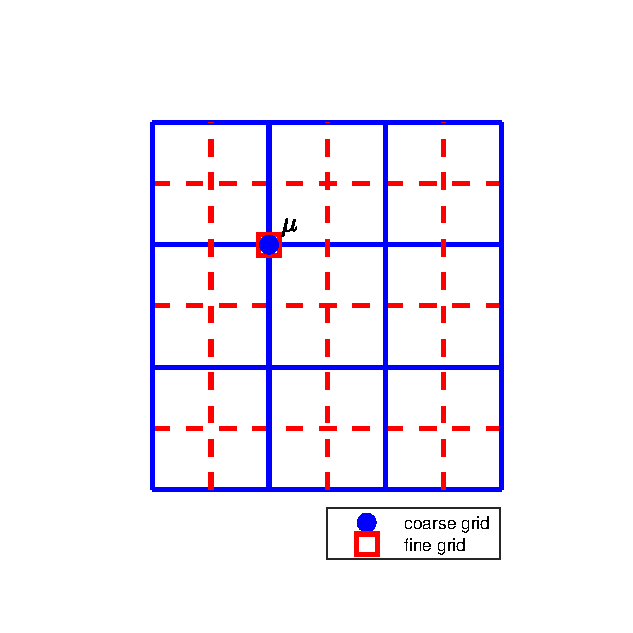
\includegraphics[width=0.24\textwidth,trim={1.8cm 0.8cm 1.4cm 1.2cm}, clip]{interpolation1.eps}
	\includegraphics[width=0.24\textwidth,trim={1.8cm 0.8cm 1.4cm 1.2cm}, clip]{interpolation2.eps}
	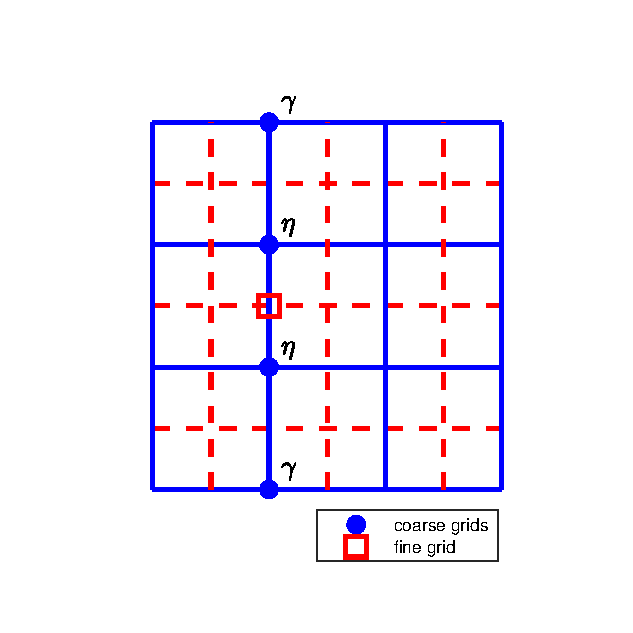
\includegraphics[width=0.24\textwidth,trim={1.8cm 0.8cm 1.4cm 1.2cm}, clip]{interpolation3.eps}
	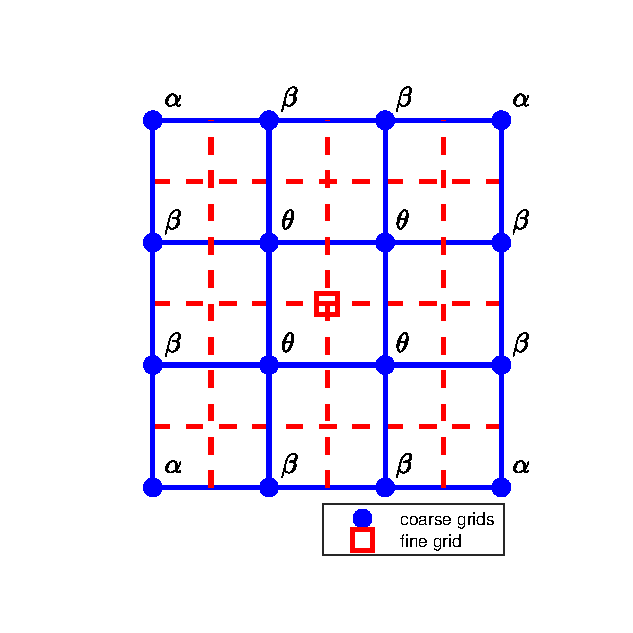
\includegraphics[width=0.24\textwidth,trim={1.8cm 0.8cm 1.4cm 1.2cm}, clip]{interpolation4.eps}
	\caption{The sketch for the stencils of fourth order interpolation operator ${\bf P}$ in two dimensions with parameters $\gamma = -\frac{1}{16}$, $\eta = \frac{9}{16}$, $\mu = 1$, $\alpha = \frac{1}{256}$, $\beta = -\frac{9}{256}$ and $\theta = \frac{81}{256}$. }\label{interpolation}
\end{figure}
\begin{figure}[htbp]
	\centering
	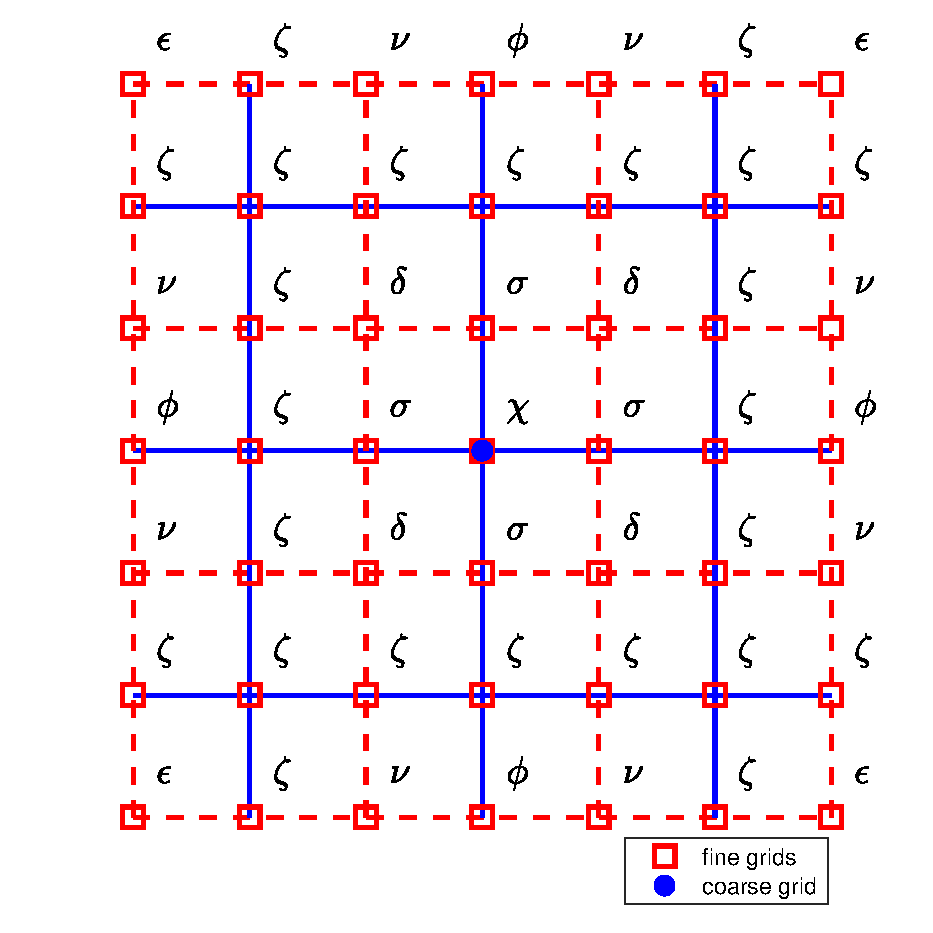
\includegraphics[width=0.6\textwidth]{restriction.eps}
	\caption{The sketch for the stencil of fourth order restriction operator ${\bf R}$ in two dimensions with parameters $\epsilon = \frac{1}{1024}$, $\nu = -\frac{9}{1024}$, $\phi = -\frac{16}{1024}$, $\delta = \frac{81}{1024}$, $\sigma = \frac{144}{1024}$, $\chi = \frac{256}{1024}$ and $\zeta = 0$.}\label{restriction}
\end{figure}






%!TEX root = elastic_3d_sbp.tex
\subsection{Boundary conditions}\label{boundary_conditions}
To conserve space, we only describe the technique for imposing boudnary conditions with ghost points. It is also possible to impose the boundary conditions without ghost points, say SAT penalty method, see \cite{?}, but we only focus on the scheme with ghost points for the boundary conditions in this paper. We only impose the boundary conditions on the top/bottom surface (direction $3$) since other boundaries are periodic; besides, we only describe the top boundary here and omit the bottom boundary. In the rest of the paper, we define a discrete scalar product as
\begin{equation}\label{scalar_product_discrete_interior}
({\bf u}, {\bf v})_h = h_1h_2h_3\sum_{i_1=1}^{n_1}\sum_{i_2=1}^{n_2}\sum_{i_3=1}^{n_3}\omega_{i_1}^{(1)}\omega_{i_2}^{(2)}\omega_{i_3}^{(3)}J_{\bf i}{\bf u}^{T}_{\bf i}{\bf v}_{\bf i}.
\end{equation}

%!TEX root = elastic_3d_sbp.tex
\subsubsection{Boundary forcing}
We start by considering the boundary forcing
\begin{equation}\label{boundary_forcing}
\mathcal{T}\cdot{\bf n}_3 = {\bf g}(x^{(1)},x^{(2)},x^{(3)},t) = (g_1,g_2,g_3)^T,
\end{equation}
where $(x^{(1)},x^{(2)},x^{(3)})$ are on the top surface and ${\bf n}_3$ is the unit outward norm of the top surface. Then in our secheme, the semi-discrtization of (\ref{elastic_equation}) and (\ref{boundary_forcing}) are
\begin{equation}\label{semi_discrete_elastic}
\rho_{\bf i}({\bf u}_{tt})_{\bf i} =\hat{L}_h{\bf u}_{\bf i}, \ \ \ t\geq0 
\end{equation}
and
\begin{equation}\label{discrete_boundary_forcing}
\frac{N_{31} D_1 {\bf u}_{{\bf i}_{\Omega_t}} + N_{32} D_2 {\bf u}_{{\bf i}_{\Omega_t}} + N_{33} \wt{D}_3 {\bf u}_{{\bf i}_{\Omega_t}}}{(J|\nabla r^{(3)}|)_{{\bf i}_{\Omega_t}}}  = {\bf g}_{i_1,i_2}, \ \ \ t\geq0.
\end{equation}
Here, $D_{1,2}$ are fourth order central difference operators for the first derivative $\partial_{1,2}$ witout using any ghost points and $\wt{D}_3$ is a fourth order SBP operator as in (\ref{sbp_1st_1}) with ghost points. Multiplying (\ref{semi_discrete_elastic}) by $h_1h_2h_3\omega_{i_1}^{(1)}\omega_{i_2}^{(2)}\omega_{i_3}^{(3)}J_{\bf i}$ and summing over all grids, we have
\begin{multline*}
({\bf u}_t,\rho{\bf u}_{tt})_h = -S_h({\bf u}_t,{\bf u}) + h_1h_2\sum_{i_1=1}^{n_1}\sum_{i_2=1}^{n_2}\omega_{i_1}^{(1)}\omega_{i_2}^{(2)}({\bf u}_t)_{{\bf i}_{\Omega_t}}^T(N_{31}D_1{\bf u}_{{\bf i}_{\Omega_t}} + N_{32}D_2{\bf u}_{{\bf i}_{\Omega_t}} +N_{33}\wt{D}_3{\bf u}_{{\bf i}_{\Omega_t}}),
\end{multline*}
where the bilinear form $S_h(\cdot,\cdot)$ is symmetric and positive semi-definite. And the equation can be rewritten as
\begin{multline}\label{time_derivative_energy}
({\bf u}_t,\rho{\bf u}_{tt})_h + S_h({\bf u}_t,{\bf u}) = 
h_1h_2\sum_{i_1=1}^{n_1}\sum_{i_2=1}^{n_2}\omega_{i_1}^{(1)}\omega_{i_2}^{(2)}({\bf u}_t)_{{\bf i}_{\Omega_t}}^T(N_{31}D_1{\bf u}_{{\bf i}_{\Omega_t}} + N_{32}D_2{\bf u}_{{\bf i}_{\Omega_t}} +N_{33}\wt{D}_3{\bf u}_{{\bf i}_{\Omega_t}}).
\end{multline}
We define the discrete energy as
\begin{equation*}
E_h := ({\bf u}_t, \rho{\bf u}_t)_h + S_h({\bf u},{\bf u}),
\end{equation*}
which is an analog of the continuous energy. 
From (\ref{time_derivative_energy}), we have
\begin{equation}\label{time_derivative_energy_2}
\frac{dE_h}{dt} = 2h_1h_2\sum_{{i_1}=1}^{n_1}\sum_{{i_2}=1}^{n_2}\omega_{i_1}^{(1)}\omega_{i_2}^{(2)}({\bf u}_t)_{{\bf i}_{\Omega_t}}^T(N_{31}D_1{\bf u}_{{\bf i}_{\Omega_t}} + N_{32}D_2{\bf u}_{{\bf i}_{\Omega_t}} +N_{33}\wt{D}_3{\bf u}_{{\bf i}_{\Omega_t}}).
\end{equation}
To obtain energy stability, we need to impose boundary forcing condition such that the right hand side of (\ref{time_derivative_energy_2}) is non-positive. Here, we use the ghost points in the direction $3$ as the additional degrees of freedom to impose the boundary forcing condition. From (\ref{discrete_boundary_forcing}), we obtain
\begin{equation}\label{eq1}
(J|\nabla r^{(3)}|)_{{\bf i}_{\Omega_t}} \left(\begin{array}{c}
(g_1)_{i_1,i_2} \\
(g_2)_{i_1,i_2}\\
(g_3)_{i_1,i_2}\end{array}\right) = \left(\begin{array}{c}
\sum_{m=1}^2\sum_{k=1}^3(N_{3m})_{1k}D_m(u_k)_{{\bf i}_{\Omega_t}} +\sum_{k=1}^3(N_{33})_{1k}\wt{D}_3(u_k)_{{\bf i}_{\Omega_t}}\\
\sum_{m=1}^2\sum_{k=1}^3(N_{3m})_{2k}D_m(u_k)_{{\bf i}_{\Omega_t}} 
+\sum_{k=1}^3(N_{33})_{2k}\wt{D}_3(u_k)_{{\bf i}_{\Omega_t}} \\
\sum_{m=1}^2\sum_{k=1}^3(N_{3m})_{3k}D_m(u_k)_{{\bf i}_{\Omega_t}}
+\sum_{k=1}^3(N_{33})_{3k}\wt{D}_3(u_k)_{{\bf i}_{\Omega_t}}
\end{array}\right),
\end{equation}
where the subscript $jk$ in $(N_{3m})_{jk}, m = 1,2,3, j,k = 1,2,3$ represents the $j^{th}$ row and $k^{th}$ column of the matrix $N_{3m}$. Then for any fixed points ${\bf i}_{\Omega_t} = (i_1,i_2,n_3)$, based on (\ref{sbp_1st_1}),
\begin{align}\label{eq2}
h_3 \tilde{D}_3(u_k)_{i_1,i_2,n_3} = -\tilde{d}_0 (u_k)_{i_1,i_2,n_3+1} - \sum_{j = 1}^4  \tilde{d}_k (u_k)_{i_1,i_2,n_3+1-k},
\end{align}
for $k = 1,2,3$. Plug (\ref{eq2}) into (\ref{eq1}), we get
\begin{align}\label{matrix_boundary}
&\hspace{0.4cm}\frac{\tilde{d}_0}{h_3}\left(\begin{array}{ccc}
(N_{33})_{11}&(N_{33})_{12} & (N_{33})_{13}\\
(N_{33})_{21} &(N_{33})_{22} &(N_{33})_{23}\\
(N_{33})_{31} &(N_{33})_{32} &(N_{33})_{33}
\end{array}\right) \left(\begin{array}{c}
(u_1)_{i_1,i_2,n_3+1}\\
(u_2)_{i_1,i_2,n_3+1}\\
(u_3)_{i_1,i_2,n_3+1}
\end{array}\right)\nonumber\\
&= \left(\begin{array}{ccc}
\sum_{m=1}^3\frac{1}{h_3}(N_{33})_{1m}\sum_{k=1}^4\tilde{d}_k(u_m)_{i_1,i_2,n_3+1-k}\\
\sum_{m=2}^3\frac{1}{h_3}(N_{33})_{2m}\sum_{k=1}^4\tilde{d}_k(u_m)_{i_1,i_2,n_3+1-k}\\
\sum_{m=2}^3\frac{1}{h_3}(N_{33})_{3m}\sum_{k=1}^4\tilde{d}_k(u_m)_{i_1,i_2,n_3+1-k}
\end{array}\right)\nonumber
+\left(\begin{array}{ccc}
\sum_{m=1}^2\sum_{k=1}^3(N_{3m})D_m(u_k)_{i_1,i_2,n_3}\\
\sum_{m=1}^2\sum_{k=1}^3(N_{3m})D_m(u_k)_{i_1,i_2,n_3}\\
\sum_{m=1}^2\sum_{k=1}^3(N_{3m})D_m(u_k)_{i_1,i_2,n_3}
\end{array}\right)\nonumber\\
&\hspace{0.4cm}-\left(\begin{array}{ccc}
(J|\nabla r^{(3)}|)_{i_1,i_2,n_3}(g_1)_{i_1,i_2}\\
(J|\nabla r^{(3)}|)_{i_1,i_2,n_3}(g_2)_{i_1,i_2}\\
(J|\nabla r^{(3)}|)_{i_1,i_2,n_3}(g_3)_{i_1,i_2}
\end{array}\right).
\end{align}
We then have the value for ghost points ${\bf u}_{i_1,i_2,n_3+1}$  after solving the linear system $(\ref{matrix_boundary})$ which is compatible with the discrete boundary focing condition (\ref{discrete_boundary_forcing}). Thus, the resulting scheme is energy conservative $\frac{dE_h}{dt} = 0$ if ${\bf g} = {\bf 0}$.


%!TEX root = elastic_3d_sbp.tex
\subsubsection{Dirichlet boundary condition}
Next, we consider the Dirichlet boundary condition, 
\begin{equation}\label{dirichlet_boundary_condition}
{\bf u}(x^{(1)},x^{(2)},x^{(3)},t) = {\bf f}(x^{(1)},x^{(2)},x^{(3)},t),  \ \ \ t \geq 0,
\end{equation}
where $(x^{(1)},x^{(2)},x^{(3)})$ are on the top surface. It is obvious that we can set ${\bf u}_{{\bf i}_{\Omega_t}} = {\bf f}_{i_1,i_2}$, but this relation does not contain any ghost points. In order to involve the ghost points, instesd (\ref{dirichlet_boundary_condition}), we consider
\begin{equation}
{\bf u}_{tt}(x^{(1)},x^{(2)},x^{(3)},t) = {\bf f}_{tt}(x^{(1)},x^{(2)},x^{(3)},t),  \ \ \ t \geq 0.
\end{equation}
From the discrete point of view, we have
\begin{equation}\label{dbc_discrete}
({\bf u}_{tt})_{{\bf i}_{\Omega_t}}=\frac{1}{\rho_{{\bf i}_{\Omega_t}}} \hat{L}_h{\bf u}_{{\bf i}_{\Omega_t}} = ({\bf f}_{tt})_{i_1,i_2}.
\end{equation}
Since we have periodic boundary conditions in the directions $1,2$ and $D_3$ in the (\ref{discrete_elastic}) use the first derivative oprator which does not contain the ghost points, the only term contains the ghost points is 
\[\frac{\hat{G}_3(N_{33}){\bf u}_{{\bf i}_{\Omega_t}}}{\rho_{{\bf i}_{\Omega_t}}J_{{\bf i}_{\Omega_t}}}.\]
Then by using (\ref{dbc_discrete}), we have the values for ghost points ${\bf u}_{i,j,n_3+1}$. Since the initial condition is compatible with the boundary condition, we can integrate (\ref{dbc_discrete}) in time once to get
\[({\bf u}_t)_{{\bf i}_{\Omega_t}} = ({\bf f}_t)_{i_1,i_2}.\]
Therefore, we have a conservative energy $\frac{dE_h}{dt} = 0$ when ${\bf f}_t = {\bf 0}$.

%!TEX root = elastic_3d_sbp.tex
\section{Grid refinement interface}
In this section, we partition the physical domian into two subdomains with interface surface $\Gamma$,
\begin{equation}\label{coarse_problem}
\rho^c\frac{\partial ^2 {\bf u}^c}{\partial t^2} =  L{\bf u}^c, \ \ \ \ \ {\bf x} \in \Omega^c,\ \ \ t>0,
\end{equation}
\begin{equation}\label{fine_problem}
\rho^f\frac{\partial ^2 {\bf u}^f}{\partial t^2} =  L{\bf u}^f, \ \ \ \ \ {\bf x} \in \Omega^f,\ \ \ t>0
\end{equation}
provided suitable initial and boundary conditions. We assume that $\Omega^f$ is on the top of $\Omega^c$ with $\Omega^c\cup\Omega^f = \Omega$ and $\Omega^c\cap\Omega^f = \Gamma=\Omega^c_t =\Omega^f_b $. The interface conditions are given to guarantee the continuity of the solutions and the continuity of the traction force,
\begin{equation}\label{continuity_sol}
{\bf u}_f = {\bf u}_c, \ \ \ \ \ \ \ \ \ \ \ \ \ \ \ \ {\bf x}\in \Gamma, \ \ \ t>0, 
\end{equation}
\begin{equation}\label{continuity_trac}
\mathcal{T}^f\cdot{\bf n}^f = -\mathcal{T}^c\cdot{\bf n}^c,  \ \ \ \ \ \ \  {\bf x}\in \Gamma, \ \ \ t>0.
\end{equation}
Dirichlet boundary condition is given on the bottom surface (direction $3$) for $\Omega^c$ and boundary forcing condition is assumed on the top surface (direction $3$) for $\Omega^f$. Directions $1$ and $2$ are periodic. By \eqref{bdry_integral_curvi}, it is easy to verify that the continuous problem \eqref{coarse_problem}-\eqref{continuity_trac} satisfies an energy estimate.

%!TEX root = elastic_3d_sbp.tex
\subsection{The fourth order SBP scheme}\label{sub_section_4_1}
We approximate the elastic wave equations (\ref{coarse_problem}) and (\ref{fine_problem}) by two different fourth order SBP schemes. For spatial discretization, we use a Cartesian mesh with mesh size $h_j^c (h_j^f)$ in the coarse domain $\Omega_c$ (fine domain $\Omega_f$) for direction $j$ with $n_j^c = 1/h_j^c +1 (n_j^f = 1/h_j^f +1), j = 1,2,3$. Suppose $(r^{c,(1)}_{i_1^c}, r^{c,(2)}_{i_2^c}, r^{c,(3)}_{i_3^c}), i_1^c = 1,2,\cdots,n_1^c, i_2^c = 1,2,\cdots,n_2^c,i_3^c=0,1,\cdots,n_3^c+1$ are grid points for domain $\Omega_c$ and   $(r^{f,(1)}_{i_1^f}, r^{f,(2)}_{i_2^f}, r^{f,(3)}_{i_3^f}), i_1^f = 1,2,\cdots,n_1^f, i_2^f = 1,2,\cdots,n_2^f,i_3^f=1,\cdots,n_3^f+1$ are grid points for domain $\Omega_f$. Note that we consider ghost points outside each boundary in direction $3$ for coarse domain $\Omega_c$; but for the fine domain $\Omega_f$, the ghost points are used only for the top surface boundary in direction $3$. Denote 
\[{\bf i}^c = (i_1^c,i_2^c,i_3^c), \ {\bf i}^c_{\Omega^c_b} = (i_1^c,i_2^c,1),\  {\bf i}^c_{\Gamma} = (i_1^c,i_2^c,n_3^c),\]
and
\[ {\bf i}^f = (i_1^f,i_2^f,i_3^f), \ {\bf i}^f_{\Gamma} = (i_1^f,i_2^f,1), \ {\bf i}^f_{\Omega_t^f} = (i_1^f,i_2^f,n_3^f).\]
Then in coarse domain $\Omega_c$, we have 
\begin{multline}\label{coarse_scheme}
\rho_{{\bf i}^c}^c ({\bf u}_{tt}^c)_{{\bf i}^c} = \frac{1}{J_{{\bf i}^c}^c}\Big[G_1^c(N_{11}^c){\bf u}_{{\bf i}^c}^c+G_2^c(N_{22}^c){\bf u}_{{\bf i}^c}^c+\uline{\wt{G}}_3^c(N_{33}^c){\bf u}_{{\bf i}^c}^c
+D_1^c(N_{12}^cD_2^c{\bf u}_{{\bf i}^c}^c)+D_1^c(N_{13}^cD_3^c{\bf u}_{{\bf i}^c}^c)
+\\D_2^c(N_{21}^cD_1^c{\bf u}_{{\bf i}^c}^c)+D_2^c(N_{23}^cD_3^c{\bf u}_{{\bf i}^c}^c)
+D_3^c(N_{31}^cD_1^c{\bf u}_{{\bf i}^c}^c)
+D_3^c(N_{32}^cD_2^c{\bf u}_{{\bf i}^c}^c)\Big] := \uline{\wt{L}}_{h^c} {\bf{u}}^c_{{\bf i}^c},
\end{multline}
For the fine domian $\Omega_f$, we impose
\begin{multline}\label{fine_scheme_2}
\rho_{{\bf i}^f}^f ({\bf u}_{tt}^f)_{{\bf i}^f} =
\frac{1}{J_{{\bf i}^f}^f}\Big[G_1^f(N_{11}^f){\bf u}_{{\bf i}^f}^f+G_2^f(N_{22}^f){\bf u}_{{\bf i}^f}^f+\wt{G}_3^f(N_{33}^f){\bf u}_{{\bf i}^f}^f
+D_1^f(N_{12}^fD_2^f{\bf u}_{{\bf i}^f}^f)+D_1^f(N_{13}^fD_3^f{\bf u}_{{\bf i}^f}^f)
+\\D_2^f(N_{21}^fD_1^f{\bf u}_{{\bf i}^f}^f)+D_2^f(N_{23}^fD_3^f{\bf u}_{{\bf i}^f}^f)
+D_3^f(N_{31}^fD_1^f{\bf u}_{{\bf i}^f}^f)+D_3^f(N_{32}^fD_2^f{\bf u}_{{\bf i}^f}^f)\Big] 
:= \wt{L}_{h^f}{\bf{u}}^f_{{\bf i}^f},
\end{multline}
with $ i_3^f = 2,\cdots,n_3^f$ and
\begin{multline}\label{fine_scheme_1}
\rho_{{\bf i}^f_{\Gamma}}^f ({\bf u}_{tt}^f)_{{\bf i}^f_{\Gamma}} = \frac{1}{J_{{\bf i}^f_{\Gamma}}^f}\Big[G_1^f(N_{11}^f){\bf u}_{{\bf i}_\Gamma^f}^f+G_2^f(N_{22}^f){\bf u}_{{\bf i}_\Gamma^f}^f
+G_3^f(N_{33}^f){\bf u}_{{\bf i}^f_{\Gamma}}^f
+D_1^f(N_{12}^fD_2^f{\bf u}_{{\bf i}^f_{\Gamma}}^f)+D_1^f(N_{13}^fD_3^f{\bf u}_{{\bf i}^f_{\Gamma}}^f)
+\\D_2^f(N_{21}^fD_1^f{\bf u}_{{\bf i}^f_{\Gamma}}^f)+
D_2^f(N_{23}^fD_3^f{\bf u}_{{\bf i}^f_{\Gamma}}^f)
+D_3^f(N_{31}^fD_1^f{\bf u}_{{\bf i}^f_{\Gamma}}^f)
+D_3^f(N_{32}^fD_2^f{\bf u}_{{\bf i}^f_{\Gamma}}^f)+{\bm \eta}_{i^f,j^f}\Big]
:= L_{h^f}{\bf u}^f_{{\bf i}^f_{\Gamma}}+{\bm \eta}_{i^f,j^f}/J^f_{{\bf i}^f_{\Gamma}},
\end{multline}
where
\begin{equation}
{\bm \eta} = \rho^f\big|_{\Gamma}\mathcal{P}\left((\rho^c)^{-1}\uline{\wt{L}}_{h^c} {\bf{u}}^c_{{\bf i}^c}\big|_{\Gamma}\right) - L_{h^f}{\bf u}^f_{{\bf i}^f_{\Gamma}}.
\end{equation}
The stencil in the interpolation operator $\mathcal{P}$ can be easily computed by a Talor series expansion. For example, consider $h_1^c = h_2^c, h_1^f = h_2^f$ and $h_1^f = \frac{1}{2}h_1^c$. Then if  $\mathcal{P}$ is a fourth order interpolation operator in $2D$, we have
\begin{align}\label{interpolation}
\left({\bf u}^f\big|_{\Gamma}\right)_{i_1^f,i_2^f} = \left(\mathcal{P} {\bf u}^c\big|_{\Gamma}\right)_{i_1^f,i_2^f} = \left\{\begin{array}{cc}
({\bf u}^c|_{\Gamma})_{(i_1^f+1)/2,(i_2^f+1)/2}, &(i_1^f,i_2^f) = (\text{odd},\text{odd}),\\
\mathcal{B}^1 ({\bf u}^c|_{\Gamma})_{i_1^f/2,(i_2^f+1)/2}, &(i_1^f,i_2^f) = (\text{even},\text{odd}),\\
\mathcal{B}^2 ({\bf u}^c|_{\Gamma})_{(i_1^f+1)/2,i_2^f/2},& (i_1^f,i_2^f) = (\text{odd},\text{even}),\\
\mathcal{B}^1\mathcal{B}^2 ({\bf u}^c|_{\Gamma})_{i_1^f/2,i_2^f/2}, & (i_1^f,i_2^f) = (\text{even},\text{even}),
\end{array}\right.
\end{align}
where $\mathcal{B}^j, j = 1,2$ are the fourth order interpolation operators in $1$D for the direction $j$.  
\begin{figure}[htbp]
	\centering
	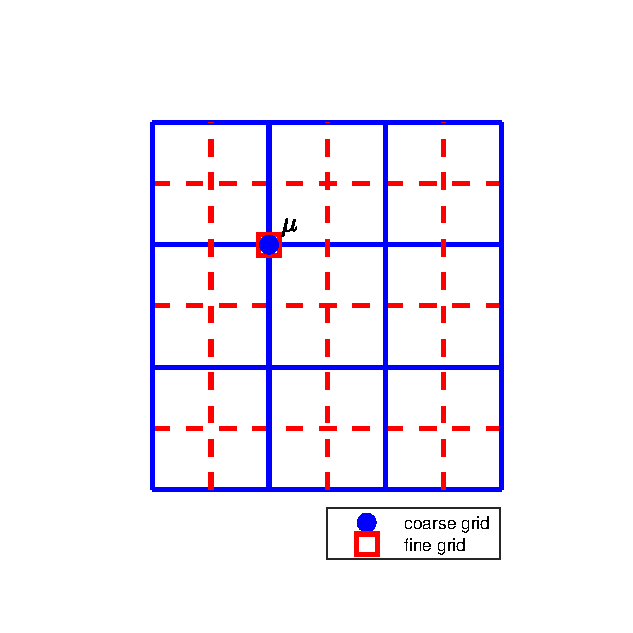
\includegraphics[width=0.45\textwidth]{interpolation1.eps}
	\includegraphics[width=0.45\textwidth]{interpolation2.eps}
	\caption{From left to right, the sketch of interpolation stencil for $(i_1^f,i_2^f) =$ (odd, odd) and $(i_1^f,i_2^f) =$ (even, odd) respectively. The number at the right-top corner are the coefficients of the corresponding coarse grids.}\label{interpolation_1_2}
\end{figure}
Figure \ref{interpolation_1_2} illustrates the interpolation coefficients when $(i_1^f,i_2^f) = $ (odd, odd) and  $(i_1^f,i_2^f) = $ (even, odd) respectively. While Figure \ref{interpolation_3_4} gives the interpolation coefficients when $(i_1^f,i_2^f) = $ (odd, even) and  $(i_1^f,i_2^f) = $ (even, even) respectively.
\begin{figure}[htbp]
	\centering
	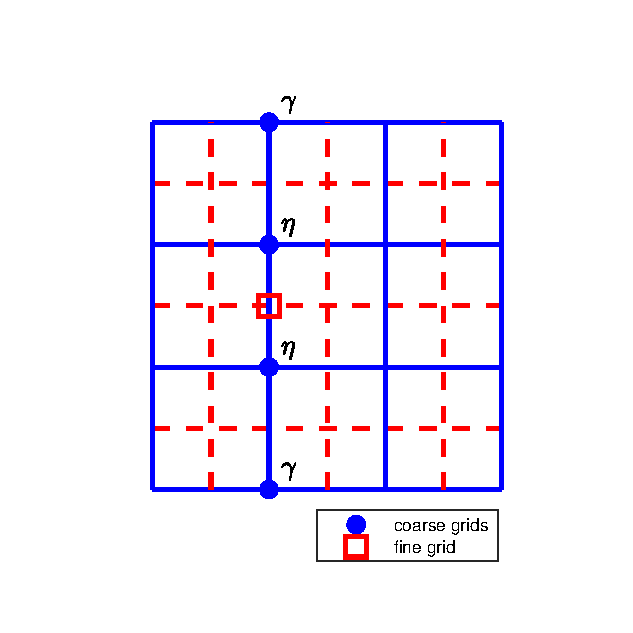
\includegraphics[width=0.45\textwidth]{interpolation3.eps}
	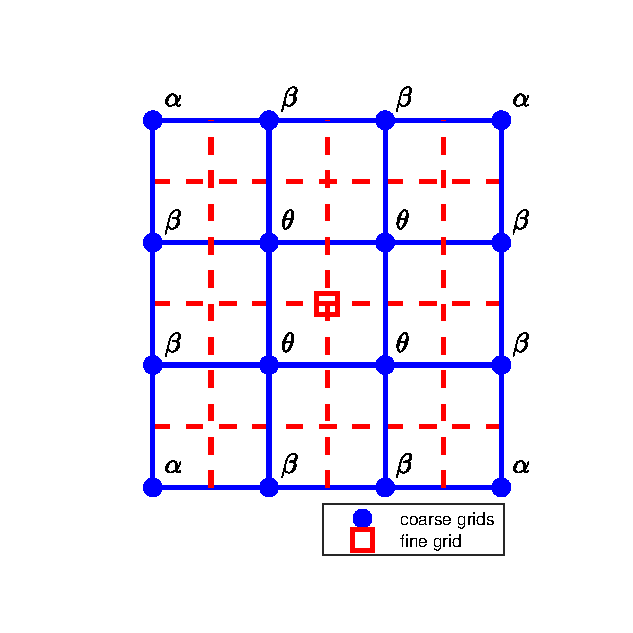
\includegraphics[width=0.45\textwidth]{interpolation4.eps}
	\caption{From left to right, the sketch of interpolation stencil for $(i_1^f,i_2^f) =$ (odd, even) and $(i_1^f,i_2^f) =$ (even, even) respectively. The number at the right-top corner are the coefficients of the corresponding coarse grids.}\label{interpolation_3_4}
\end{figure}

Furthermore, the compatibility condition of the intrpolation operator $\mathcal{P}$ and restriction operator $\mathcal{R}$, $\mathcal{P} = 4\mathcal{R}^T$ for $h_1^c = 2h_1^f$ in $2$D, determines the corresponding restriction operator $\mathcal{R}$ with
\begin{equation}\label{restriction}
({\bf u}^c|_{\Gamma})_{i^c,j^c} = (\mathcal{R}{\bf u}^f|_{\Gamma})_{i^c,j^c} = \mathcal{A}^2\mathcal{A}^1 ({\bf u}^f|_{\Gamma})_{2i^c-1,2j^c-1},
\end{equation}
where $\mathcal{A}^j, j = 1,2$ are the fourth order restriction operators in $1$D for the direction $j$. Figure \ref{extrapolation} shows the restriction coefficients for the coarse grids $(i_1^c,i_2^c)$.

\begin{figure}[htbp]
	\centering
	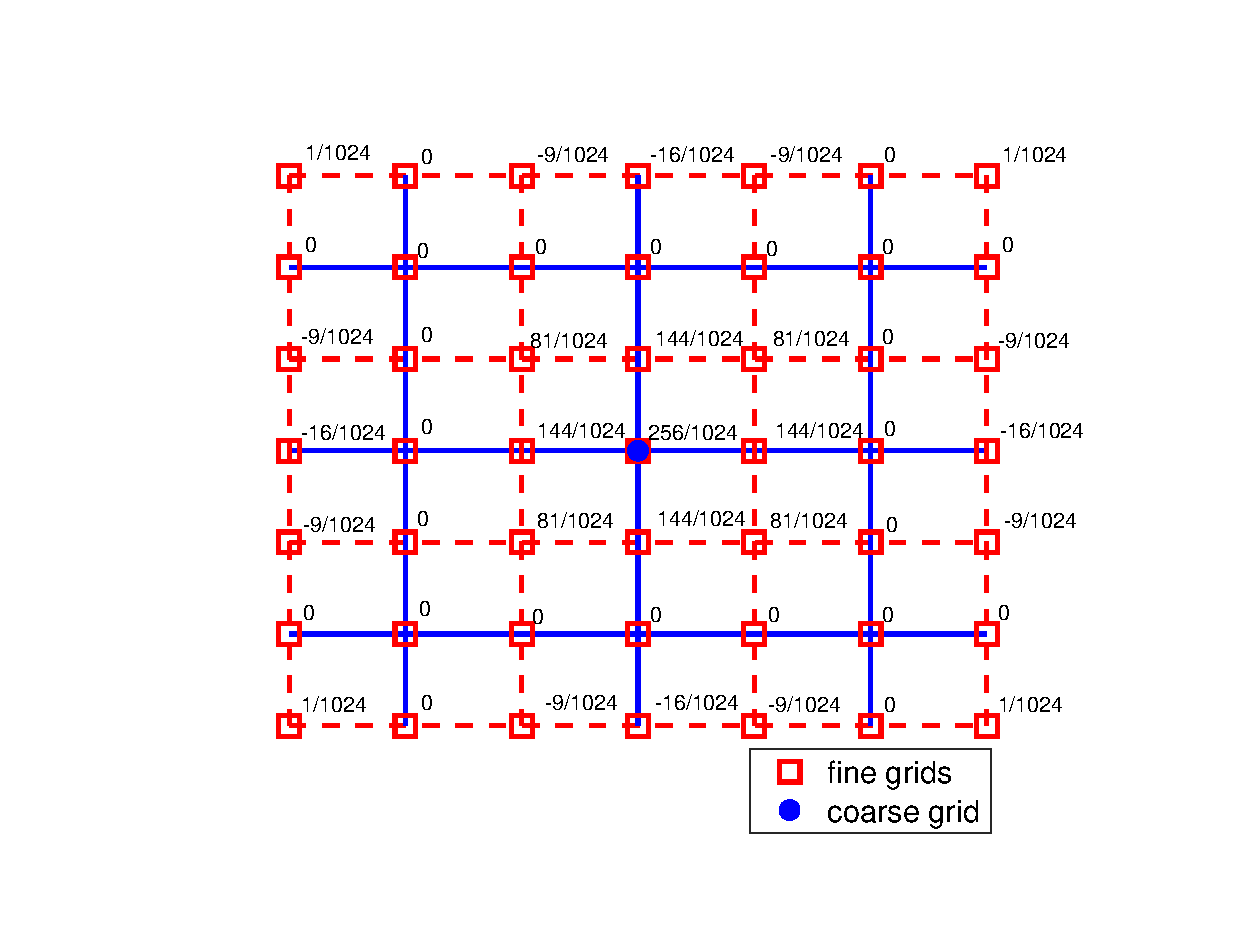
\includegraphics[width=0.8\textwidth]{restriction1.eps}
	\caption{The sketch of restriction operator in $2$D. The number at the right-top corner are the coefficients of the corresponding fine grids.}\label{extrapolation}
\end{figure}
For the simplicity of analysis, we introduce a general notation for the schemes (\ref{fine_scheme_2}) and (\ref{fine_scheme_1}) in the fine domain $\Omega_f$,
\begin{align}\label{fine_scheme}
\rho^f_{{\bf i}^f} ({\bf u}_{tt}^f)_{{\bf i}^f} = \hat{L}_{h^f}{\bf u}^f_{{\bf i}^f} =  \left\{
\begin{aligned}
&\wt{L}_{h^f}{\bf{u}}^f_{{\bf i}^f}, \ \ i_3^f = 2,3,\cdots,n_3^f,\\
&L_{h^f}{\bf u}^f_{{\bf i}^f_{\Gamma}}+{\bm \eta}_{i^f,j^f}/J^f_{{\bf i}^f_{\Gamma}},
\end{aligned}
\right.
\end{align}
For the grids in the fine domain $\Omega^f$  that are lying on the interface $\Gamma$, we impose the continuity of the solution,
\begin{equation}\label{data_continuous_curvi}
{\bf u}^f\big|_{\Gamma} = \mathcal{P}\big({\bf u}^c\big|_{\Gamma}\big).
\end{equation}
As for the ghost points which are close to the top surface of the coarse domian, we impose the continuity of the traction force,
\begin{equation}\label{traction_continuous_curvi}
{\bf n}^c\cdot\mathcal{T}^c \big|_\Gamma = \mathcal{R}\left(-{\bf n}^f\cdot\mathcal{T}^f\big|_\Gamma - \frac{h_3^f\omega_1^{(3)}{\bm \eta}}{J^f\big|\nabla r_f^{(3)}\big|}\Bigg|_\Gamma\right).
\end{equation}

%!TEX root = elastic_3d_sbp.tex
\subsection{Energy estimate}
In this section, we investigate the energy estimate for the semi-discrete forms (\ref{elastic_semi_c}) and (\ref{fine_scheme}) in section \ref{semi_discrete_form}. Provided periodic boundary conditions in directions $1$ and $2$. Let ${\bf u}, {\bf v}$ be grid functions in $\Omega^c$. We define the three dimensional scalar product in $\Omega^c$
\begin{equation}\label{scalar_product_inner}
({\bf u}, {\bf v})_{2h} = 8h_1h_2h_3\sum_{i=1}^{n_1^{2h}}\sum_{j=1}^{n_2^{2h}}\sum_{k=1}^{n_3^{2h}}\omega_k{J}_{ijk}^{2h}u_{ijk}v_{ijk},
\end{equation}
where $J^{2h}_{ijk}$ located at the $((k-1)n_1^{2h}n_2^{2h}+(j-1)n_1^{2h}+i)$'th row and $((k-1)n_1^{2h}n_2^{2h}+(j-1)n_1^{2h}+i)$'th column of ${\bf J}^{2h}$, $u_{ijk}$ and $v_{ijk}$ loacted at the $((k-1)n_1^{2h}n_2^{2h}+(j-1)n_1^{2h}+i)$'th row of ${\bf u}$, ${\bf v}$ repectively. The two dimensional scalar product for grid functions on the interface $\Gamma^c$
\begin{equation}\label{scalar_product_discrete_interface_c}
\left<{\bf u}_{\Gamma^c}, {\bf v}_{\Gamma^c}\right>_{2h} = 4h_1h_2\sum_{i=1}^{n_1^{2h}}\sum_{j=1}^{n_2^{2h}}{ J}_{\Gamma,ij}^{2h}\big|\nabla_x^c r^{3}\big|_{ij}u_{ij}v_{ij}.
\end{equation}
with $J^{2h}_{\Gamma,ij}$ located at the $((j-1)n_1^{2h}+i)$'th row and $((j-1)n_1^{2h}+i)$'th column of diagonal matrix ${\bf J}_{\Gamma}^{2h}$, $u_{ij}$, $v_{ij}$ are the $((j-1)n_1^{2h}+i)$'th element of $u_{\Gamma^c}$ and $v_{\Gamma^f}$ respectively. On the other hand, let ${\bf u}, {\bf v}$ be grid functions in $\Omega^f$. We define the three dimensional discrete scalar product in $\Omega^f$ similarly as in $\Omega^c$
\begin{equation*}
({\bf u}, {\bf v})_{h} = h_1h_2h_3\sum_{i=1}^{n_1^{h}}\sum_{j=1}^{n_2^{h}}\sum_{k=1}^{n_3^{h}}\omega_k{J}_{ijk}^{h}u_{ijk}v_{ijk},
\end{equation*}
and the two dimensional scalar product for grid functions on the interface $\Gamma^f$
\begin{equation}\label{scalar_product_discrete_interface_f}
\left<{\bf u}_{\Gamma^f}, {\bf v}_{\Gamma^f}\right>_{h} = h_1h_2\sum_{i=1}^{n_1^{h}}\sum_{j=1}^{n_2^{h}}{ J}^{h}_{\Gamma,ij}\big|\nabla_x^f r^{3}\big|_{ij}u_{ij}v_{ij},
\end{equation}
where $J^h_{ijk}$, $u_{ijk}$, $v_{ijk}$, $J^h_{\Gamma,ij}$, $u_{ij}$ and $v_{ij}$ have similar definitions as in (\ref{scalar_product_inner}) and (\ref{scalar_product_discrete_interface_c}).

 Now, we are ready to present the energy conservation of the proposed schemes in Section \ref{semi_discrete_form}. Multiplying (\ref{elastic_semi_c}) by $8h_1h_2h_3\omega_k{\mathcal J}^{2h}{\bf c}_t$ and summing over all grids, we have
\begin{equation}\label{coarse_simple}
({\bf c}_t, {\varrho}^{2h}{\bf c}_{tt})_{2h} = ({\bf c}_t,\wt{L}^{2h}\wt{{\bf c}})_{2h} = -S_{2h}({\bf c}_t,{\bf c}) + B_{2h}({\bf c}_t,\wt{{\bf c}}),
\end{equation}
multiplying (\ref{fine_scheme}) by $h_1h_2h_3\omega_k{\mathcal J}^h{\bf f}_t$ and summing over all grids, we obtain
\begin{equation*}
({\bf f}_t, {\varrho}^h{\bf f}_{tt})_h = ({\bf f}_t,\hat{L}^h{\bf f})_h = -S_h({\bf f}_t,{\bf f}) + B_h({\bf f}_t,{\bf f}) 
+h_1h_2h_3\omega_1({\bf f}_\Gamma)_t^T{\bm \eta},
\end{equation*}
where  both $S_{2h}$ and $S_h$ are symmetric and positive definite bilinear forms, and 
\begin{equation}\label{boundary_f}
B_h ({\bf f}_t,{\bf f}) = -h_1h_2({\bf f}_{\Gamma})_t^T\big(\mathcal{N}_{31}^h{\mathcal D}_1^h {\bf f}\big|_{\Gamma}+ \mathcal{N}_{32}^h\mathcal{D}_2^h{\bf f}\big|_{\Gamma}+\mathcal{N}_{33}^h\mathcal{D}_3^h{\bf f}\big|_{\Gamma}\big),
\end{equation}
and
\begin{equation}\label{bounary_c}
B_{2h} ({\bf c}_t,\wt{\bf c}) = 4h_1h_2({\bf c}_{\Gamma})_t^T\big(\mathcal{N}_{31}^{2h}\mathcal{D}_1^{2h}{\bf c}\big|_{\Gamma}+ \mathcal{N}_{32}^{2h}\mathcal{D}_2^{2h}{\bf c}\big|_{\Gamma}+\mathcal{N}_{33}^{2h}\wt{\mathcal{D}}_3^{2h}\wt{{\bf c}}\big|_{\Gamma}\big).
\end{equation}
Then, the time derivative of the semi-discrete energy reads as
\begin{multline}\label{semi_energy_1}
\frac{d}{dt}\big[({\bf f}_t,\varrho^h {\bf f}_t)_h + S_h({\bf f},{\bf f}_t) + ({\bf c}_t,\varrho^{2h} {\bf c}_t)_{2h} + S_{2h}({\bf c},{\bf c}_t) \big]  = \\
2B_{h}({\bf f}_t,{\bf f}) + 2B_{2h}({\bf c}_t,\wt{\bf c}) + 2h_1h_2h_3\omega_1({\bf f}_\Gamma)_t^T{\bm \eta},
\end{multline}
plugging (\ref{boundary_f})--(\ref{bounary_c}) into (\ref{semi_energy_1}) and combining the definition of the scalar product on the interface $\Gamma$ (\ref{scalar_product_discrete_interface_c})--(\ref{scalar_product_discrete_interface_f}), we have
\begin{align*}\label{semi_energy_2}
&\hspace{0.4cm}\frac{d}{dt}\left[({\bf f}_t,\varrho^h {\bf f}_t)_{h} + S_{h}({\bf f},{\bf f}_t) + ({\bf c}_t,\varrho^{2h} {\bf c}_t)_{2h} + S_{2h}({\bf c},{\bf c}_t) \right]   \nonumber\\
& = 2\left<({\bf f}_\Gamma)_t,|\nabla^f r^{3}|^{-1}(\mathcal{J}^h_\Gamma)^{-1}(-\mathcal{A}_3^h{\bf f}\big|_\Gamma+h\omega_1{\bm \eta})\right>_{h}+ 2\left<({\bf c}_\Gamma)_t,|\nabla^c r^{3}|^{-1}(\mathcal{J}^{2h}_\Gamma)^{-1}\wt{\mathcal{A}}_3^{2h}\wt{\bf c}\big|_\Gamma\right>_{2h} \nonumber\\
& = 2\left<\wt{\mathcal{P}}\big(({\bf c}_\Gamma)_t\big),|\nabla^f r^{3}|^{-1}(\mathcal{J}^h_\Gamma)^{-1}(-\mathcal{A}_3^h{\bf f}\big|_\Gamma+h\omega_1{\bm \eta})\right>_{h}+ 2\left<({\bf c}_\Gamma)_t,|\nabla^c r^{3}|^{-1}(\mathcal{J}^{2h}_\Gamma)^{-1}\wt{\mathcal{A}}_3^{2h}\wt{\bf c}\big|_\Gamma\right>_{2h} \nonumber\\
& = 2\left<({\bf c}_\Gamma)_t,\wt{\mathcal{R}}\big(|\nabla^f r^{3}|^{-1}(\mathcal{J}^h_\Gamma)^{-1}(-\mathcal{A}_3^h{\bf f}\big|_\Gamma+h\omega_1{\bm \eta})\big)\right>_{2h}+ 2\left<({\bf c}_\Gamma)_t,|\nabla^c r^{3}|^{-1}(\mathcal{J}^{2h}_\Gamma)^{-1}\wt{\mathcal{A}}_3^{2h}\wt{\bf c}\big|_\Gamma\right>_{2h} = 0,
\end{align*}
where we have used the notaions in (\ref{hatAf})--(\ref{hatAc}).


%!TEX root = SISC_elastic_3d.tex
\section{The temporal discretization}
The equations are advanced in time with an explicit fourth order accurate predictor-corrector time integration method. Like all explicit time stepping methods, the time step must not exceed the CFL stability limit. By a similar analysis as in \cite{sjogreen2012fourth}, we require 
\begin{equation*}
\Delta_t\leq C_{\text{cfl}}\min\{h_1,h_2,h_3\}/\sqrt{\kappa_{\max}},
\end{equation*}
where $C_{\text{cfl}} = 1.3$ and
$\kappa_{\text{max}}$ is the maximum eigenvalue of the matrices 
\[T_{\bf i}^{\{f,c\}} = \frac{1}{\rho^{\{f,c\}}({\bf r}_{\bf i})}\left(\begin{array}{ccc}
Tr(N_{11}^{\{f,c\}}({\bf r}_{\bf i})) &  Tr(N_{12}^{\{f,c\}}({\bf r}_{\bf i}))& Tr(N_{13}^{\{f,c\}}({\bf r}_{\bf i}))\\
Tr(N_{21}^{\{f,c\}}({\bf r}_{\bf i})) & Tr(N_{22}^{\{f,c\}}({\bf r}_{\bf i})) & Tr(N_{23}^{\{f,c\}}({\bf r}_{\bf i}))\\
Tr(N_{31}^{\{f,c\}}({\bf r}_{\bf i})) & Tr(N_{32}^{\{f,c\}}({\bf r}_{\bf i})) & Tr(N_{33}^{\{f,c\}}({\bf r}_{\bf i}))\end{array}\right), \]
where $Tr(N_{lm}^{\{f,c\}}({\bf r}_{\bf i}))$ represents the trace of $3\times3$ matrix $N_{lm}^{\{f,c\}}({\bf r}_{\bf i})$. Note that $\kappa_{\text{max}}$ is related to the material properties $\mu^{\{f,c\}}, \lambda^{\{f,c\}}$ and $\rho^{\{f,c\}}$. The notation $\{\cdot,\cdot\}$ represents the component-wise identities. In the following, we give detailed procedures about how we apply the fourth order time integrator to the semidiscretizations (\ref{elastic_semi_c}) and  (\ref{fine_scheme}). 

Let ${\bf c}^{n}$ and ${\bf f}^{n}$ denote the numerical approximations of ${\bf c}({\bf x},t_n), {\bf x}\in\Omega^c$ and ${\bf f}({\bf x},t_n), {\bf x}\in\Omega^f$, respectively. Here, $t_n = n\Delta_t, n = 0,1,\cdots$ and $\Delta_t > 0$ is a constant time step. We present the fourth order time integrator with predictor and corrector in  Algorithm \ref{first_alg}.
~\\
\begin{breakablealgorithm}
	\caption{Fourth order accurate time stepping for the semidiscretizations  (\ref{elastic_semi_c}) and  (\ref{fine_scheme}). }\label{first_alg}
	Given  $\wt{{\bf c}}^{n}, \wt{{\bf c}}^{n-1}$ and ${\bf f}^{n}, {\bf f}^{n-1}$ that satisfy the discretized interface conditions.
	
	\begin{itemize}
		\item  {Compute the predictor at the interior grid points %for both fine and coarse domains
			\[{\bf c}^{*,n+1}_{\bf i} = 2{\bf c}^{n}_{\bf i} - {\bf c}^{n-1}_{\bf i} + \Delta_t^2\left((\rho^{2h}\otimes{\bf I})(J^{2h}\otimes{\bf I})\right)^{-1}{\wt{\mathcal{L}}}^{2h}_{\bf i} {\bf{c}}^{n},\quad {\bf i}\in I_{\Omega^c},\]
			\[{\bf f}^{*,n+1}_{\bf i} = 2{\bf f}^{n}_{\bf i} - {\bf f}^{n-1}_{\bf i} + \Delta_t^2\left((\rho^{h}\otimes{\bf I})(J^{h}\otimes{\bf I})\right)^{-1}\hat{\mathcal{L}}^{h}_{\bf i} {\bf{f}}^{n},\quad {\bf i}\in I_{\Omega^f}\backslash I_{\Gamma^f}.\]
		}
		\item{At the interface $\Gamma$, the values ${\bf f}^{*,n+1}_{\bf i}$  are computed by the continuity of solution 
			\begin{equation*}
			{\bf f}^{*,n+1}_{\bf i} = {\mathcal{P}}_{\bf i}({\bf c}^{*,n+1}),\quad {\bf i}\in I_{\Gamma^f}.
			\end{equation*}
		}
		\item{At the interface $\Gamma$, the ghost point values in $\wt{\bf c}^{*,n+1}$ are computed by solving the equation for the continuity of traction 
			%\begin{equation}\label{traction_gamma_pre}
			%({\Lambda}^{c}_{{\bf i}'}{J}_{{\bf i}'}^{c})^{-1}\wt{\mathcal{A}}_3^{2h}{\bf c}^{*,n+1}_{{\bf i}'}
			%= {\mathcal{R}}\left(({\Lambda}^{f}_{\bf i}{J}^f_{\bf i})^{-1}(\mathcal{A}_3^h{\bf f}^{*,n+1}_{\bf i}-h_3\omega_1{\bm \eta}^{\ast,n+1}_{\bf i})\right),\quad {\bf i}'\in I_{\Gamma^c},\quad {\bf i}\in I_{\Gamma^f}.
			%\end{equation}
				\begin{equation}\label{traction_gamma_pre}
			\left(\left((\Lambda^{2h}J^{2h}_{\Gamma})\otimes{\bf I}\right)^{-1}\wt{\mathcal{A}}_3^{2h}{\bf c}^{\star,n+1}\right)_{\bf i}
			= {\mathcal{R}}_{\bf i}\Big(\left((\Lambda^hJ_{\Gamma}^h)\otimes{\bf I}\right)^{-1}(\mathcal{A}_3^h{\bf f}^{\star,n+1}-h_3\omega_1{\bm \eta}^{\star,n+1})\Big), {\bf i}\in I_{\Gamma^c}.
			\end{equation}
		}
		\item{Evaluate the acceleration at all grid points 
			\begin{equation*}
			\underline{\wt{\bf c}}^n= \frac{\wt{\bf c}^{*,n+1}-2\wt{\bf c}^{n}+\wt{\bf c}^{n-1}}{\Delta^2_t},\ \ \ \
			\underline{{\bf f}}^{n} = \frac{{\bf f}^{*,n+1}-2{\bf f}^{n}+{\bf f}^{n-1}}{\Delta^2_t}.
			\end{equation*}
		}
		\item{Compute the corrector at the interior grid points
			\[{\bf c}^{n+1}_{\bf i} = {\bf c}^{*,n+1}_{\bf i} + \frac{\Delta_t^4}{12}\left((\rho^{2h}\otimes{\bf I})(J^{2h}\otimes{\bf I})\right)^{-1}\wt{\mathcal{L}}^{2h}_{\bf i}\underline{{\bf{c}}}^{n},\quad {\bf i}\in I_{\Omega^c},\]
			\[{\bf f}^{n+1}_{\bf i} = {\bf f}^{*,n+1}_{\bf i} + \frac{\Delta_t^4}{12}\left((\rho^{h}\otimes{\bf I})(J^h\otimes{\bf I})\right)^{-1}\hat{\mathcal{L}}^{h}_{\bf i}\underline{{\bf{f}}}^{n},\quad {\bf i}\in I_\Omega^f.\]
		}
		\item{At the interface $\Gamma$, the values ${\bf f}^{n+1}_{\bf i}$  are computed by the continuity of solution
			\begin{equation*}
			{\bf f}^{n+1}_{\bf i} = {\mathcal{P}}_{\bf i}({\bf c}^{n+1}), \quad {\bf i}\in I_{\Gamma^f}.
			\end{equation*}
		}
		\item{At the interface $\Gamma$, the ghost point values in $\wt{\bf c}^{n+1}$ are computed by solving the equation for the continuity of traction
			\begin{equation}\label{traction_gamma_corr}
			%({\Lambda}^{c}_{{\bf i}'}{J}_{{\bf i}'}^{c})^{-1}(\wt{\mathcal{A}}_3^{2h}{\bf c}^{n+1}_{{\bf i}'})
			%= {\mathcal{R}}\left(({\Lambda}^{f}_{\bf i}{ J}^f_{\bf i})^{-1}((\mathcal{A}_3^h{\bf f}^{n+1}_{\bf i})-h_3\omega_1{\bm \eta}^{n+1}_{\bf i})\right), \quad {{\bf i}'}\in I_{\Gamma^c}, \quad {\bf i}\in I_{\Gamma^f}.
			\left(\left((\Lambda^{2h}J^{2h}_{\Gamma})\otimes{\bf I}\right)^{-1}\wt{\mathcal{A}}_3^{2h}{\bf c}^{n+1}\right)_{\bf i}
			= {\mathcal{R}}_{\bf i}\Big(\left((\Lambda^hJ^h_{\Gamma})\otimes{\bf I}\right)^{-1}(\mathcal{A}_3^h{\bf f}^{n+1}-h_3\omega_1{\bm \eta}^{n+1})\Big), \quad {\bf i}\in I_{\Gamma^c}.
			\end{equation}
		}
	\end{itemize}
\end{breakablealgorithm}
~\\

In the Algorithm \ref{first_alg}, we need to solve the linear systems for the continuity of traction at the interface $\Gamma$ in both predictor step (\ref{traction_gamma_pre}) and corrector step (
\ref{traction_gamma_corr}). The linear system matrices of (\ref{traction_gamma_pre}) and (\ref{traction_gamma_corr}) are the same. Therefore, we only present how to solve (\ref{traction_gamma_pre}) in the predictor step.

There are $3n_1^{2h}n_2^{2h}$ unknowns and $3n_1^{2h}n_2^{2h}$ linear equations in (\ref{traction_gamma_pre}). For large problems in three dimensions, it is very memory inefficient to calculate the LU-factorization. Therefore, we use iterative methods to solve the linear system in (\ref{traction_gamma_pre}). In particular, we consider three different iterative methods: the block Jacobi iterative method, the conjugate gradient (CG) iterative method and the preconditioned conjugate gradient iterative method. The detailed methods and a comparison are given in Section \ref{iterative_section}.

%!TEX root = SISC_elastic_3d.tex
%\subsection{Time discretization with SBP scheme}
In the following, we give detailed procedures about how we apply the fourth order time integrator to the problems (\ref{elastic_semi_c}) and  (\ref{fine_scheme}). 

Let ${\bf c}^{n}$ and ${\bf f}^{n}$ denote the numerical approximations of ${\bf C}({\bf x},t_n), {\bf x}\in\Omega^c$ and ${\bf F}({\bf x},t_n), {\bf x}\in\Omega^f$ respectively. Here, $t_n = n\Delta_t, n = 0,1,\cdots$ and $\Delta_t > 0$ is a constant time step. We present the fourth order time integrator with predictor and corrector in  Algorithm \ref{first_alg}.
~\\
\begin{breakablealgorithm}
	\caption{Fourth order accurate time stepping for the semi-discretization .......}\label{first_alg}
	Given  $\wt{{\bf c}}^{n}, \wt{{\bf c}}^{n-1}$ and ${\bf f}^{n}, {\bf f}^{n-1}$ that satisfy the discretized interface conditions.
	
	\begin{itemize}
		\item  {Compute the predictor at the interior grid points for both fine and coarse domains
			\begin{equation*}
			{\bf c}^{*,n+1} = 2{\bf c}^{n} - {\bf c}^{n-1} + \Delta_t^2(\varrho^{2h})^{-1}{\wt{\mathcal{L}}}^{2h} \wt{\bf{c}}^{n},\ \ \ 
			{\bf f}^{*,n+1} = 2{\bf f}^{n} - {\bf f}^{n-1} + \Delta_t^2(\varrho^h)^{-1}\hat{\mathcal{L}}^{h} {\bf{f}}^{n}.
			\end{equation*}
		}
		\item{For the continuity of solution on the interface $\Gamma$, assign the value ${\bf f}_{\Gamma}^{*,n+1}$ to satisfy
			\begin{equation*}
			{\bf f}^{*,n+1}_{\Gamma} = \wt{\mathcal{P}}\big({\bf c}^{*,n+1}_{\Gamma}\big).
			\end{equation*}
		}
		\item{For the continuity of traction on the interface $\Gamma$, assign the ghost points value in $\wt{\bf c}^{*,n+1}$ to satisfy
			\begin{equation}\label{traction_gamma_pre}
			(\bm{\Lambda}^{2h}{\mathcal J}_{\Gamma}^{2h})^{-1}(\wt{\mathcal{A}}_3^{2h}\wt{\bf c}^{*,n+1})\big|_\Gamma
			= \wt{\mathcal{R}}\left((\bm{\Lambda}^{h}{\mathcal J}^h_{\Gamma})^{-1}((\mathcal{A}_3^h{\bf f}^{*,n+1})\big|_\Gamma-h_3\omega_1{\bm \eta}^{\ast,n+1})\right)
			\end{equation}
			with the definition of $\wt{\mathcal{A}}_3^{2h}$ in (\ref{hatAc}), and $\mathcal{A}_3^h$ in (\ref{hatAf}) .
		}
		\item{Evaluate the acceleration at all grids 
			\begin{equation*}
			\wt{\bf c}^n= \frac{\wt{\bf c}^{*,n+1}-2\wt{\bf c}^{n}+\wt{\bf c}^{n-1}}{\Delta^2_t},\ \ \ \
			{\bf f}^{n} = \frac{{\bf f}^{*,n+1}-2{\bf f}^{n}+{\bf f}^{n-1}}{\Delta^2_t},
			\end{equation*}
		}
		\item{Compute the corrector at the interior grid points
			\begin{equation*}
			{\bf c}^{n+1} = {\bf c}^{*,n+1} + \frac{\Delta_t^4}{12}(\varrho^{2h})^{-1}\wt{\mathcal{L}}^{2h}\wt{\bf{c}}^{n},\ \ \ 
			{\bf f}^{n+1} = {\bf f}^{*,n+1} + \frac{\Delta_t^4}{12}(\varrho^{h})^{-1}\hat{\mathcal{L}}^{h}{\bf{f}}^{n}.
			\end{equation*}
		}
		\item{For the continuity of solution on the interface $\Gamma$, assign the value ${\bf f}^{n+1}_\Gamma$ to satisfy
			\begin{equation*}
			{\bf f}^{n+1}_{\Gamma} = \wt{\mathcal{P}}\big({\bf c}^{n+1}_{\Gamma}\big).
			\end{equation*}
		}
		\item{For the continuity of traction on the interface $\Gamma$, assign the ghost point value in $\wt{\bf c}^{n+1}$ to satisfy
			\begin{equation}\label{traction_gamma_corr}
			(\bm{\Lambda}^{2h}{\mathcal J}_{\Gamma}^{2h})^{-1}(\wt{\mathcal{A}}_3^{2h}\wt{\bf c}^{n+1})\big|_\Gamma
			= \wt{\mathcal{R}}\left((\bm{\Lambda}^{h}{\mathcal J}^h_{\Gamma})^{-1}((\mathcal{A}_3^h{\bf f}^{n+1})\big|_\Gamma-h_3\omega_1{\bm \eta}^{n+1})\right)
			\end{equation}
			with the definition of $\wt{\mathcal{A}}_3^{2h}$ in (\ref{hatAc}), and $\mathcal{A}_3^h$ in (\ref{hatAf}).
		}
	\end{itemize}
\end{breakablealgorithm}
~\\
%Here, we only give the steps to evolve the elastic wave equation with suitable initial and interface conditions and skip the detailed derivations of the fourth order predictor corrector time integrator. For more details, see  \cite{wang2018fourth}.

In the Algorithm \ref{first_alg}, we need to solve the equations from the continuity of the traction force for the interface $\Gamma$ in both predictor step (\ref{traction_gamma_pre}) and corrector step (
\ref{traction_gamma_corr}). The structure of (\ref{traction_gamma_pre}) and (\ref{traction_gamma_corr}) are the same, for simplicity, we only clarify how we solve (\ref{traction_gamma_pre}) in the predictor step.

There are $3n_1^{2h}n_2^{2h}$ unknowns in (\ref{traction_gamma_pre}) and $3n_1^{2h}n_2^{2h}$ linear equations in (\ref{traction_gamma_pre}). For large problems in three dimension, it is very memory inefficient to calculate the LU-factorization. Therefore, We use iterative methods to solve the linear system (\ref{traction_gamma_pre}). In particular, we consider three different iterative methods: block Jacobi iterative method, conjugate gradient iterative method and preconditioned conjugate gradient iterative method. The details are given in Section \ref{iterative_section}.


%!TEX root = elastic_3d_sbp.tex
\section{Numerical Experiments}
In this section, we conduct several numerical experiments. In Section \ref{manufactured_sol}, we compare the efficiency of iterative methods which are used to solve the interface condition system (\ref{traction_gamma_pre}) and (\ref{traction_gamma_corr}), note that the coefficient matrices in (\ref{traction_gamma_pre}) and (\ref{traction_gamma_corr}) are same; verify the order of the convergence of the proposed scheme (\ref{elastic_semi_c}), (\ref{fine_scheme}) and (\ref{continuous_sol})--(\ref{continuous_traction}). In Section \ref{gaussian_source}, we show that there is no obvious reflection at the mesh refinment interface for the proposed scheme (\ref{elastic_semi_c}), (\ref{fine_scheme}) and (\ref{continuous_sol})--(\ref{continuous_traction}) with only a traction force on the top surface. Finally, the energy conservation property is shown in Section \ref{conserved_energy}.

%!TEX root = elastic_3d_sbp.tex
\subsection{Method of manufactured solutions}\label{manufactured_sol}
We take the computation domain to be 
\begin{equation}\label{coarse_domain_manufactured}
\left\{
\begin{aligned}
& x^{c,1} = 2\pi r^1\\
& x^{c,2} = 2\pi r^2\\
& x^{c,3} = r^3\theta_i\big(r^1,r^2\big) + (1-r^3)\theta_b\big(r^1,r^2\big)
\end{aligned}
\right.
\end{equation}
for coarse domain $\Omega^c$. Here, $0\leq r^1, r^2, r^3\leq 1$, $f_i$ is the interface surface geometry,
\begin{equation}\label{iterface_geometry}
\theta_i\big(r^1,r^2\big) = \pi+0.2\sin(4\pi r^1)+0.2\cos(4\pi r^2),
\end{equation}
and 
$\theta_b$ is the bottom surface geometry,
\begin{equation}\label{bottom_geometry}
\theta_b\big(r^1,r^2\big) = 0.2\exp\left(-\frac{(r^1-0.6)^2}{0.04}\right)+0.2\exp\left(-\frac{(r^2-0.6)^2}{0.04}\right).
\end{equation}
As for the fine domian $\Omega^f$, it is chosen to be
\begin{equation}\label{fine_domain_manufactured}
\left\{
\begin{aligned}
& x^{f,1} = 2\pi r^1\\
& x^{f,2} = 2\pi r^2\\
& x^{f,3} = r^3\theta_t\big(r^1,r^2\big) + (1-r^3)\theta_i\big(r^1,r^2\big),
\end{aligned}
\right.
\end{equation}
where $0\leq r^1, r^2, r^3\leq 1$, $\theta_t$ is the top surface geometry,
\begin{equation}\label{top_geometry}
\theta_t\big(r^1,r^2\big) = 0.2\exp\left(-\frac{(r^1-0.5)^2}{0.04}\right)+0.2\exp\left(-\frac{(r^2-0.5)^2}{0.04}\right),
\end{equation}
and $\theta_i$ is the interface geometry which is given in (\ref{iterface_geometry}). Note that the subdomian 
$\Omega^f$ is on the top of the subdomain $\Omega^c$. For both fine and coarse domians, let the density vary according to
\begin{equation}\label{density_function}
\rho(x^1,x^2,x^3) = 2 + \sin(x^1+0.3)\sin(x^2+0.3)\sin(x^3-0.2),
\end{equation}
and material parameters $\mu, \lambda$ satisfy
\begin{equation}\label{mu_function}
\mu(x^1,x^2,x^3) = 3 + \sin(3x^1+0.1)\sin(3x^2+0.1)\sin(x^3),
\end{equation}
and 
\begin{equation}\label{lambda_function}
\lambda(x^1,x^2,x^3)  = 21+ \cos(x^1+0.1)\cos(x^2+0.1)\sin^2(3x^3),
\end{equation}
respectively. Besides, we impose a boundary forcing on the top surface and Dirichlet boundary conditions for the other boundaries. The external forcing, top boundary forcing ${\bf g}$ and initial conditions are chosen such that ${\bf u}(\cdot,t) = (u_1(\cdot,t),u_2(\cdot,t),u_3(\cdot,t))^T$ with
\begin{align*}
u_1(\cdot,t) &= \cos(x^1+0.3)\sin(x^2+0.3)\sin(x^3+0.2)\cos(t^2),\\
u_2(\cdot,t) &= \sin(x^1+0.3)\cos(x^2+0.3)\sin(x^3+0.2)\cos(t^2),\\
u_3(\cdot,t) &= \sin(x^1+0.2)\sin(x^2+0.2)\cos(x^3+0.2)\sin(t).
\end{align*}
For example, for the boundary forcing on the top surface, we impose 
\begin{equation}\label{traction_force}
{\bf g} = (g_1,g_2,g_3)^T = \sum_{i=1}^3\left(\sum_{j = 1}^3 M_{ij}^f\frac{\partial{\bf u}}{\partial x^{(j)}}\right) n^{f,+,i}_3,
\end{equation}
where, $M_{ij}^f$ and $n^{f,+,i}_3 $ can be found in (\ref{M_definition}) and (\ref{outward_normal}) respectively.

%!TEX root = SISC_elastic_3d.tex
\subsection{Iterative methods}\label{iterative_section}
In this section, we use the same example as in Sec.~\ref{convergence_study}. For the proposed scheme (\ref{elastic_semi_c}, \ref{fine_scheme}, \ref{continuous_sol}, \ref{continuous_traction}), we need to solve a $3n_1^{2h}n_2^{2h}\times 3n_1^{2h}n_2^{2h}$ linear system at each time step twice for the continuity of traction at the interface $\Gamma$. 

We investigate three iterative methods: the block Jacobi method, the conjugate gradient method, and the preconditioned conjugate gradient method. We note that the coefficient matrix of the linear system arising from the continuity of traction at interface $\Gamma$ is not symmetric positive definite for this test problem. However, our experiment shows that both the conjugate gradient method and the preconditioned conjugate gradient method converge. Except the following test that compares the three iterative methods, we always use the block Jacobi method to guarantee that the whole scheme converges. 

For the problem proposed in Sec.~\ref{convergence_study}, the structure of the coefficient matrix of the linear system arising in (\ref{continuous_traction}) is shown in Figure \ref{Mass_matrix}, which is determined by the interpolation operator ${\mathcal{P}}$ and restriction operator ${\mathcal{R}}$. Here, we use $n_1^{2h} = n_2^{2h}=13, n_3^{2h} = 7$ as an example. We choose the red parts in Figure \ref{Mass_matrix} to be the block Jacobi matrix in block Jacobi iterative method and preconditioning matrix in preconditioned conjugate gradient iterative method. The absolute error tolerance is set to be $1e-7$ for all three iterative methods and $h_1 = h_2 = h_3 = h$.

\begin{table}[htbp]
	\begin{center}
		\begin{tabular}{|c|c c c|}
			\hline
			$2h$   & ~~~~ CG ~~~~& Block Jacobi & Preconditioned CG  \\
			\hline
			$2\pi/24$ &37.78& 24.96& 4.01\\
			\hline
			$2\pi/48$ &38.61 & 25.38 & 2.87\\
			\hline 
			$2\pi/96$ &39.14 &25.43 & 2.25\\
			\hline
		\end{tabular}
	\end{center}
	\caption{Condition number of matrices in conjugate gradient method, block Jacobi method and preconditioned conjugate gradient method}\label{condition_number}
\end{table} 
Table \ref{condition_number} shows the condition number of the original coefficient matrix, the block Jacobi matrix and the coefficient matrix after applying the preconditioner, respectively. We observe that the condition number for preconditioned conjugate gradient method is smallest which is consistent with the results of iteration number for different iterative methods: there are around $44$ iterations for conjugate gradient method, $13$ iterations for block Jacobi method and $9$ iterations for preconditioned conjugate gradient method.

In comparison, we have also performed an LU factorization for the linear system when the mesh size $2h = 2\pi/96$, and the computation takes 40.6 GB memory. In contrast, with the block Jacobi method, the peak memory usage is only 1.2 GB. For large-scale problems, the memory usage becomes infeasible for the LU factorization. 

\begin{figure}[H]
	\centering
	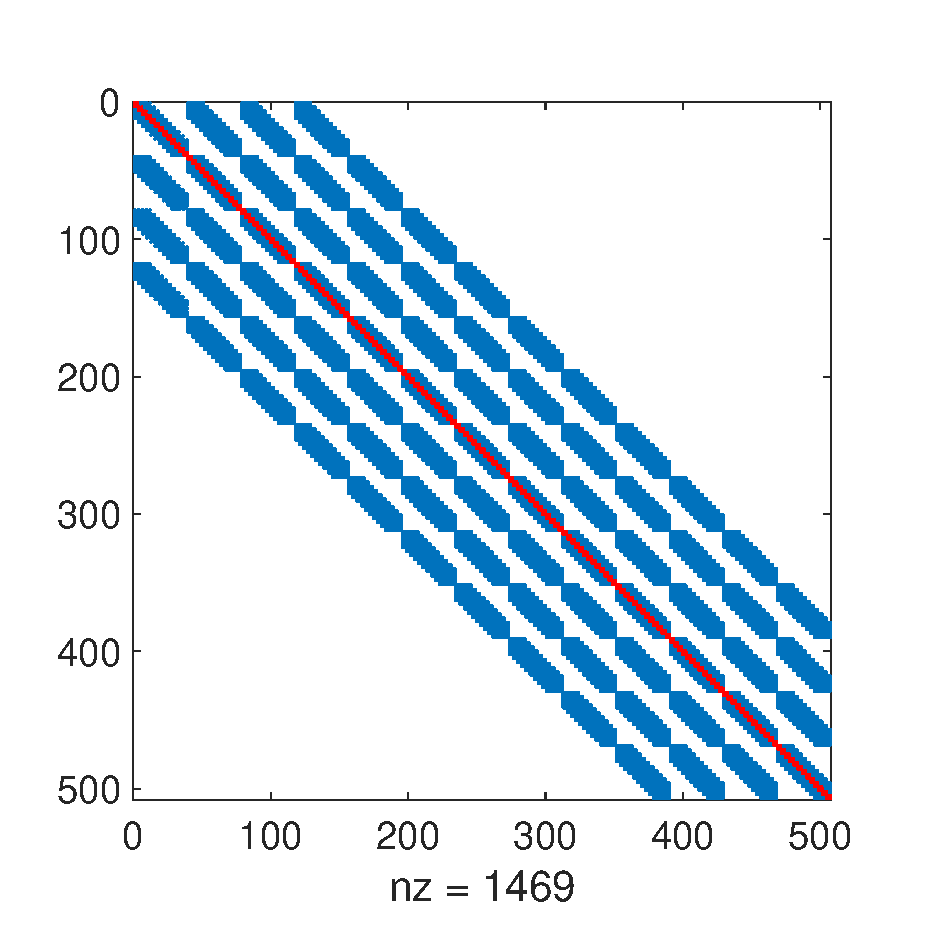
\includegraphics[width=0.45\textwidth,trim={0.6cm 1cm 1cm 1.2cm}, clip]{Mass_matrix.eps}
	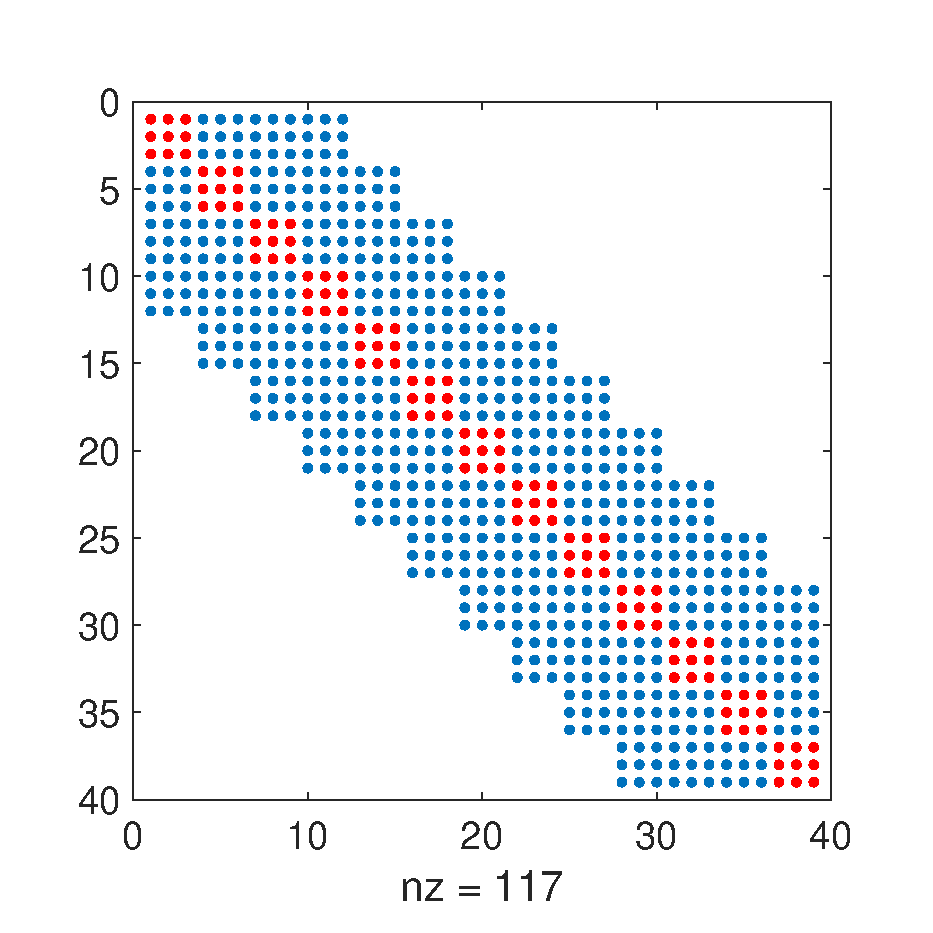
\includegraphics[width=0.45\textwidth,trim={0.6cm 1cm 1cm 1.2cm}, clip]{Mass_diagonal_matrix.eps}
	\caption{The left panel is the structure of the coefficient matrix of the linear system (\ref{continuous_traction}).  The right panel shows a close-up of one diagonal block.}\label{Mass_matrix}
\end{figure}


%!TEX root = elastic_3d_sbp.tex
\subsubsection{Verification of convergence rate}\label{convergence_study}
We now perform a convergence study for the proposed scheme (\ref{coarse_scheme})--(\ref{traction_continuous_curvi}). The convergence rate is computed by
\[log\left(\frac{e_h}{e_{2h}}\right)\Bigg/log\left(\frac{1}{2}\right),\]
here, $e_h$ is the corresponding $L^2$ error.  The $L^2$ error for the numerical solutions in the whole domain, $L^{f,2}$ error for the numerical solutions in the fine domain $\Omega^f$ and$L^{c,2}$ error for the numerical solutions in the coarse domain $\Omega^c$ are presented in Table \ref{convergence_rate}. We observe that the convergence rate is fourth order for all cases, thought the theoretical convergence rate is second for the points near boundaries. Note that we use a block Jacobian iterative method for the experiments here.

\begin{table}[htb]
	\begin{center}
		\begin{tabular}{|c|c c c|}
			\hline
			$h^c = 2h^f$   & $L^2$ & $L^{f,2}$ & $L^{c,2}$  \\
			\hline
			$2\pi/24$ &1.7740e-03 ~~~~~~~~ & 8.8534e-04 ~~~~~~~~ & 1.5373e-03 ~~~~~~~~\\
			\hline
			$2\pi/48$ &1.0658e-04 (4.06) & 5.5352e-05 (4.00) & 9.1084e-05 (4.08)\\
			\hline 
			$2\pi/96$ &6.3379e-06 (4.07) & 3.2694e-06 (4.08) & 5.4296e-06 (4.07)\\
			\hline
		\end{tabular}
	\end{center}
	\caption{Convergence rate of the fourth order SBP method}\label{convergence_rate}
\end{table} 


%!TEX root = SISC_elastic_3d.tex
\subsection{Gaussian source}\label{gaussian_source}
In this section, we perform a numerical simulation with a Gaussian source at the top surface and verify that  the curved mesh refinement interface does not generate obvious artifacts. 

We choose a flat top and bottom surface geometry 
\begin{equation*}
\theta_t\big(r^{(1)},r^{(2)}\big) = 1000,\quad \theta_b\big(r^{(1)},r^{(2)}\big) = 0,
\end{equation*}
respectively. The mesh refinement interface is parameterized by
\begin{equation}\label{interface_gausian}
\theta_i\big(r^{(1)},r^{(2)}\big) = 800+20\sin(4\pi r^{(1)})+20\cos(4\pi r^{(2)}),
\end{equation}
where $0\leq r^{(1)}, r^{(2)}, r^{(3)}\leq 1$. 
In addition, the mapping in the coarse domain $\Omega^c$ and fine domain $\Omega^f$ are given by 
\[ {\bf x} = {\bf X}^c({\bf r}) = \left(\begin{array}{c}
2000 r^{(1)}\\
2000 r^{(2)}\\
r^{(3)} \theta_i\big(r^{(1)}, r^{(2)}\big) + (1-r^{(3)}) \theta_b\big(r^{(1)},r^{(2)}\big) \end{array}\right) \]
and 
\[ {\bf x} = {\bf X}^f({\bf r}) = \left(\begin{array}{c}
2000 r^{(1)}\\
2000 r^{(2)}\\
r^{(3)}\theta_t\big(r^{(1)},r^{(2)}\big) + (1-r^{(3)})\theta_i\big(r^{(1)},r^{(2)}\big)\end{array}\right), \]
respectively. 
%For the coarse domain $\Omega^c$, the mapping is given by
%\[ {\bf x} = {\bf X}^c({\bf r}) = \left(\begin{array}{c}
%2000 r^{(1)}\\
%2000 r^{(2)}\\
%r^{(3)} \theta_i\big(r^{(1)}, r^{(2)}\big) + (1-r^{(3)}) \theta_b\big(r^{(1)},r^{(2)}\big) \end{array}\right). \]
%Here, $0\leq r^{(1)}, r^{(2)}, r^{(3)}\leq 1$, $\theta_i$ represents the interface surface geometry,
%\begin{equation}\label{interface_gausian}
%\theta_i\big(r^{(1)},r^{(2)}\big) = 800+20\sin(4\pi r^{(1)})+20\cos(4\pi r^{(2)}),
%\end{equation}
%and $\theta_b$ is the bottom surface geometry,
%\begin{equation*}
%\theta_b\big(r^{(1)},r^{(2)}\big) = 0.
%\end{equation*}
%As for the fine domain $\Omega^f$, the mapping is chosen to be
%\[ {\bf x} = {\bf X}^f({\bf r}) = \left(\begin{array}{c}
%2000 r^{(1)}\\
%2000 r^{(2)}\\
%r^{(3)}\theta_t\big(r^{(1)},r^{(2)}\big) + (1-r^{(3)})\theta_i\big(r^{(1)},r^{(2)}\big)\end{array}\right), \]
%where $0\leq r^{(1)}, r^{(2)}, r^{(3)}\leq 1$ and $\theta_t$ is the top surface geometry with
%\begin{equation*}
%\theta_t\big(r^{(1)},r^{(2)}\big) = 1000,
%\end{equation*}
%$\theta_i$ is the interface geometry which is given in (\ref{interface_gausian}). 
In the entire domain, we use the homogeneous material properties
%\begin{equation*}
%\rho(x^{(1)},x^{(2)},x^{(3)}) = 1.5\times 10^3,
%\end{equation*}
%and 
\begin{equation*}
\rho(x^{(1)},x^{(2)},x^{(3)}) = 1.5\times 10^3,\ \  \mu(x^{(1)},x^{(2)},x^{(3)}) = 1.5\times 10^9,\ \ 
\lambda(x^{(1)},x^{(2)},x^{(3)})  = 3\times 10^9.
\end{equation*}
At the top surface, the Gaussian source 
${\bf g} = (g_1,g_2,g_3)^T$ is imposed as Dirichlet data with $g_1 = g_2 = 0$ and 
\[g_3 = 10^9 \text{exp}\left(-\left(\frac{t-4/44.2}{1/44.2}\right)^2\right)\text{exp}\left(-\left(\frac{x^{(1)}-1000}{12.5}\right)^2-\left(\frac{x^{(2)}-1000}{12.5}\right)^2\right).\]  
Homogeneous Dirichlet boundary conditions are imposed at other boundaries. Both the initial conditions and the external forcing are set to zero everywhere.% and the initial conditions are also set to be zero everywhere, ${\bf F}(\cdot,0) = {\bf C}(\cdot,0) = {\bf u}(\cdot,0) = {\bf 0}, {\bf u}(\cdot,t) = (u_1(\cdot,t), u_2(\cdot,t), u_3(\cdot,t))^T$.

In the numerical schemes, we consider three different meshes: Mesh 1 is the Cartesian mesh without any interface and $n_1 = n_2 = 201, n_3 = 101$ with $n_i$ denotes the number of grid points in the direction $x^{(i)}$. This corresponds to 10 grid points per wavelength and is considered as the  reference solution. Mesh 2 is the curvilinear mesh with a curved mesh refinement interface defined in \eqref{interface_gausian} and $n_1^{2h} = n_2^{2h} = 101, n_3^{2h} = 41$, $n_1^h = n_2^h = 201, n_3^h = 21$. The mesh size in $\Omega^f$ is approximately the same as the mesh size in the Cartesian mesh. As a result, the waves are resolved with 5 grid points per wavelength in $\Omega^c$. Mesh 3 is obtained by refining Mesh 2 in all three spatial directions. %The final simulation time is $T = 0.4$. %is a curvilinear mesh with the same curved mesh refinement interface and $n_1^{2h} = n_2^{2h} = 201, n_3^{2h} = 81$, $n_1^h = n_2^h = 401, n_3^h = 41$. We notice that the third mesh is a finer version of the second mesh. The final simulation time is $T = 0.4$.

\begin{figure}[htbp]
	\centering
	\includegraphics[width=0.49\textwidth,trim={0.05cm 0.1cm 0.55cm 0.45cm}, clip]{u1_t02_cartesian.png}
	\includegraphics[width=0.49\textwidth,trim={0.05cm 0.1cm 0.55cm 0.45cm}, clip]{u1_t04_cartesian.png}\\
	\includegraphics[width=0.49\textwidth,trim={0.05cm 0.1cm 0.55cm 0.45cm}, clip]{u1_t02_curvi.png}
	\includegraphics[width=0.49\textwidth,trim={0.05cm 0.1cm 0.55cm 0.45cm}, clip]{u1_t04_curvi.png}\\
	\includegraphics[width=0.49\textwidth,trim={0.05cm 0.1cm 0.55cm 0.45cm}, clip]{u1_t02_curvi_finer.png}
	\includegraphics[width=0.49\textwidth,trim={0.05cm 0.1cm 0.55cm 0.45cm}, clip]{u1_t04_curvi_finer.png}
\caption{The graphs for $u_1$. In the top, middle and bottom panel, we show numerical solutions at $t=0.2$ and $t=0.4$ computed with Mesh 1, Mesh 2 and Mesh 3, respectively. The curved interfaces are marked with the red dash lines.}
\label{u1}
\end{figure}

%\begin{figure}[htbp]
%	\centering
%	\includegraphics[width=0.4\textwidth,trim={0 2.8cm 0 2.8cm}, clip]{u2_t02_cartesian.png}
%	\includegraphics[width=0.4\textwidth,trim={0 2.8cm 0 2.8cm}, clip]{u2_t02_curvi_mr.png}\\
%	\includegraphics[width=0.4\textwidth,trim={0 2.8cm 0 2.8cm}, clip]{u2_t04_cartesian.png}
%	\includegraphics[width=0.4\textwidth,trim={0 2.8cm 0 2.8cm}, clip]{u2_t04_curvi_mr.png}
%	\caption{The graph for $u_2$. From left to right are for Cartesian mesh without mesh refinement interface and curvilinear mesh with mesh refinement interface respectively. From top to bottom are for $t = 0.2$ and $t = 0.4$ respectively. Note that $x,z$ in the graph correspond to $x^{(1)}, x^{(3)}$ respectively.}\label{u2}
%\end{figure}

\begin{figure}[htbp]
	\centering
	\includegraphics[width=0.49\textwidth,trim={0.05cm 0.1cm 0.55cm 0.45cm}, clip]{u3_t02_cartesian.png}
	\includegraphics[width=0.49\textwidth,trim={0.05cm 0.1cm 0.55cm 0.45cm}, clip]{u3_t04_cartesian.png}\\
	\includegraphics[width=0.49\textwidth,trim={0.05cm 0.1cm 0.55cm 0.45cm}, clip]{u3_t02_curvi.png}
	\includegraphics[width=0.49\textwidth,trim={0.05cm 0.1cm 0.55cm 0.45cm}, clip]{u3_t04_curvi.png}\\
	\includegraphics[width=0.49\textwidth,trim={0.05cm 0.1cm 0.55cm 0.45cm}, clip]{u3_t02_curvi_finer.png}
	\includegraphics[width=0.49\textwidth,trim={0.05cm 0.1cm 0.55cm 0.45cm}, clip]{u3_t04_curvi_finer.png}
	\caption{The graphs for $u_3$. In the top, middle and bottom panel, we show numerical solutions at $t=0.2$ and $t=0.4$ computed with Mesh 1, Mesh 2 and Mesh 3, respectively. The curved interfaces are marked with the red dash lines.}
\label{u3}
\end{figure}
In Figure \ref{u1}, we plot the component $u_1$ at $t=0.2$ and $t=0.4$.  Some artifacts are observed in the solution computed with the second mesh, which is due to the small number of grid points per wavelength in $\Omega^c$. The results become better when the finer curvilinear mesh is used. From Figure \ref{u3}, we observe that there is no obvious reflection at the mesh refinement interface for the component $u_3$, and we have a better results when a finer curvilinear mesh is used. The component $u_2$ is zero up to round-off error for both the Cartesian mesh and curvilinear meshes and is not presented here.

%!TEX root = SISC_elastic_3d.tex
\subsection{Energy conservation test}\label{conserved_energy}
To verify the energy conservation property of our scheme, we perform a computation without external source term, but with a Gaussian initial profile which centered at the origin of the computational domain.  Specifically, the computational domain, density function $\rho$ and material functions $\mu, \lambda$ are taken to be the same as in the Section \ref{convergence_study}; the initial Gaussian profiles are
\begin{align*}
	u_1(\cdot,0) &= \mbox{exp}\left(-\frac{(x^1-\pi)^2}{0.1}\right)\mbox{exp}\left(-\frac{(x^2-\pi)^2}{0.1}\right)\mbox{exp}\left(-\frac{(x^3-\pi)^2}{0.1}\right),\\
	u_2(\cdot,0) &= \mbox{exp}\left(-\frac{(x^1-\pi)^2}{0.2}\right)\mbox{exp}\left(-\frac{(x^2-\pi)^2}{0.2}\right)\mbox{exp}\left(-\frac{(x^3-\pi)^2}{0.2}\right),\\
	u_3(\cdot,0) &= \mbox{exp}\left(-\frac{(x^1-\pi)^2}{0.1}\right)\mbox{exp}\left(-\frac{(x^2-\pi)^2}{0.2}\right)\mbox{exp}\left(-\frac{(x^3-\pi)^2}{0.2}\right).
\end{align*}
Energy conservation is ensured by homogeneous Dirichlet boundary conditions. The grid spacing is $h_1 = h_2 = h_3 = h$ and $2h = \frac{\pi}{24}$ for coarse domain $\Omega^c$, $h = \frac{\pi}{48}$ for fine domain $\Omega^f$, thus we have $25\times25\times13$ grid points in the coarse domain $\Omega^c$ and $49\times49\times25$ grid points in the fine domain $\Omega^f$. 

For the semi-discrete approximation, the energy is given by $({\bf f}_t,\mathcal{\varrho}^h{\bf f}_t)_h + S_h({\bf f},{\bf f}_t) + ({\bf c}_t,\mathcal{\varrho}^{2h}{\bf c}_t)_{2h} + S_{2h}({\bf c},{\bf c}_t)$, see (\ref{semi_energy_1}). By using a same approach as for the isotropic elastic wave equation, see \cite{petersson2015wave,sjogreen2012fourth},  the expression for the fully discrete energy reads as
\begin{align*}
E^{n+1/2} &= \left|\left|\sqrt{\mathcal{\varrho}^h}\frac{{\bf f}^{n+1}-{\bf f}^n}{\Delta t}\right|\right|_h^2 + S_h({\bf f}^{n+1},{\bf f}^n) - \frac{(\Delta t)^2}{12}(\mathcal{L}^h{\bf f}^{n+1},\mathcal{L}^h{\bf f}^n)_h\\
&+ \left|\left|\sqrt{\mathcal{\varrho}^{2h}}\frac{{\bf c}^{n+1}-{\bf c}^n}{\Delta t}\right|\right|_{2h}^2 + S_{2h}({\bf c}^{n+1},{\bf c}^n) - \frac{(\Delta t)^2}{12}(\wt{\mathcal{L}}^{2h}\wt{\bf c}^{n+1},\wt{\mathcal{L}}^{2h}\wt{\bf c}^n)_{2h}.
\end{align*}
We present the relative change in fully discrete energy, $(E^{n+1/2}-E^{1/2})/E^{1/2}$, as a function of time with $t\in[0,90]$ in Figure \ref{discrete_energy}. This corresponds to $6186$ time steps. Our numerical results show that the fully discrete energy remains constant up to $4e-14$ relative error. 
\begin{figure}[htbp]
	\centering
	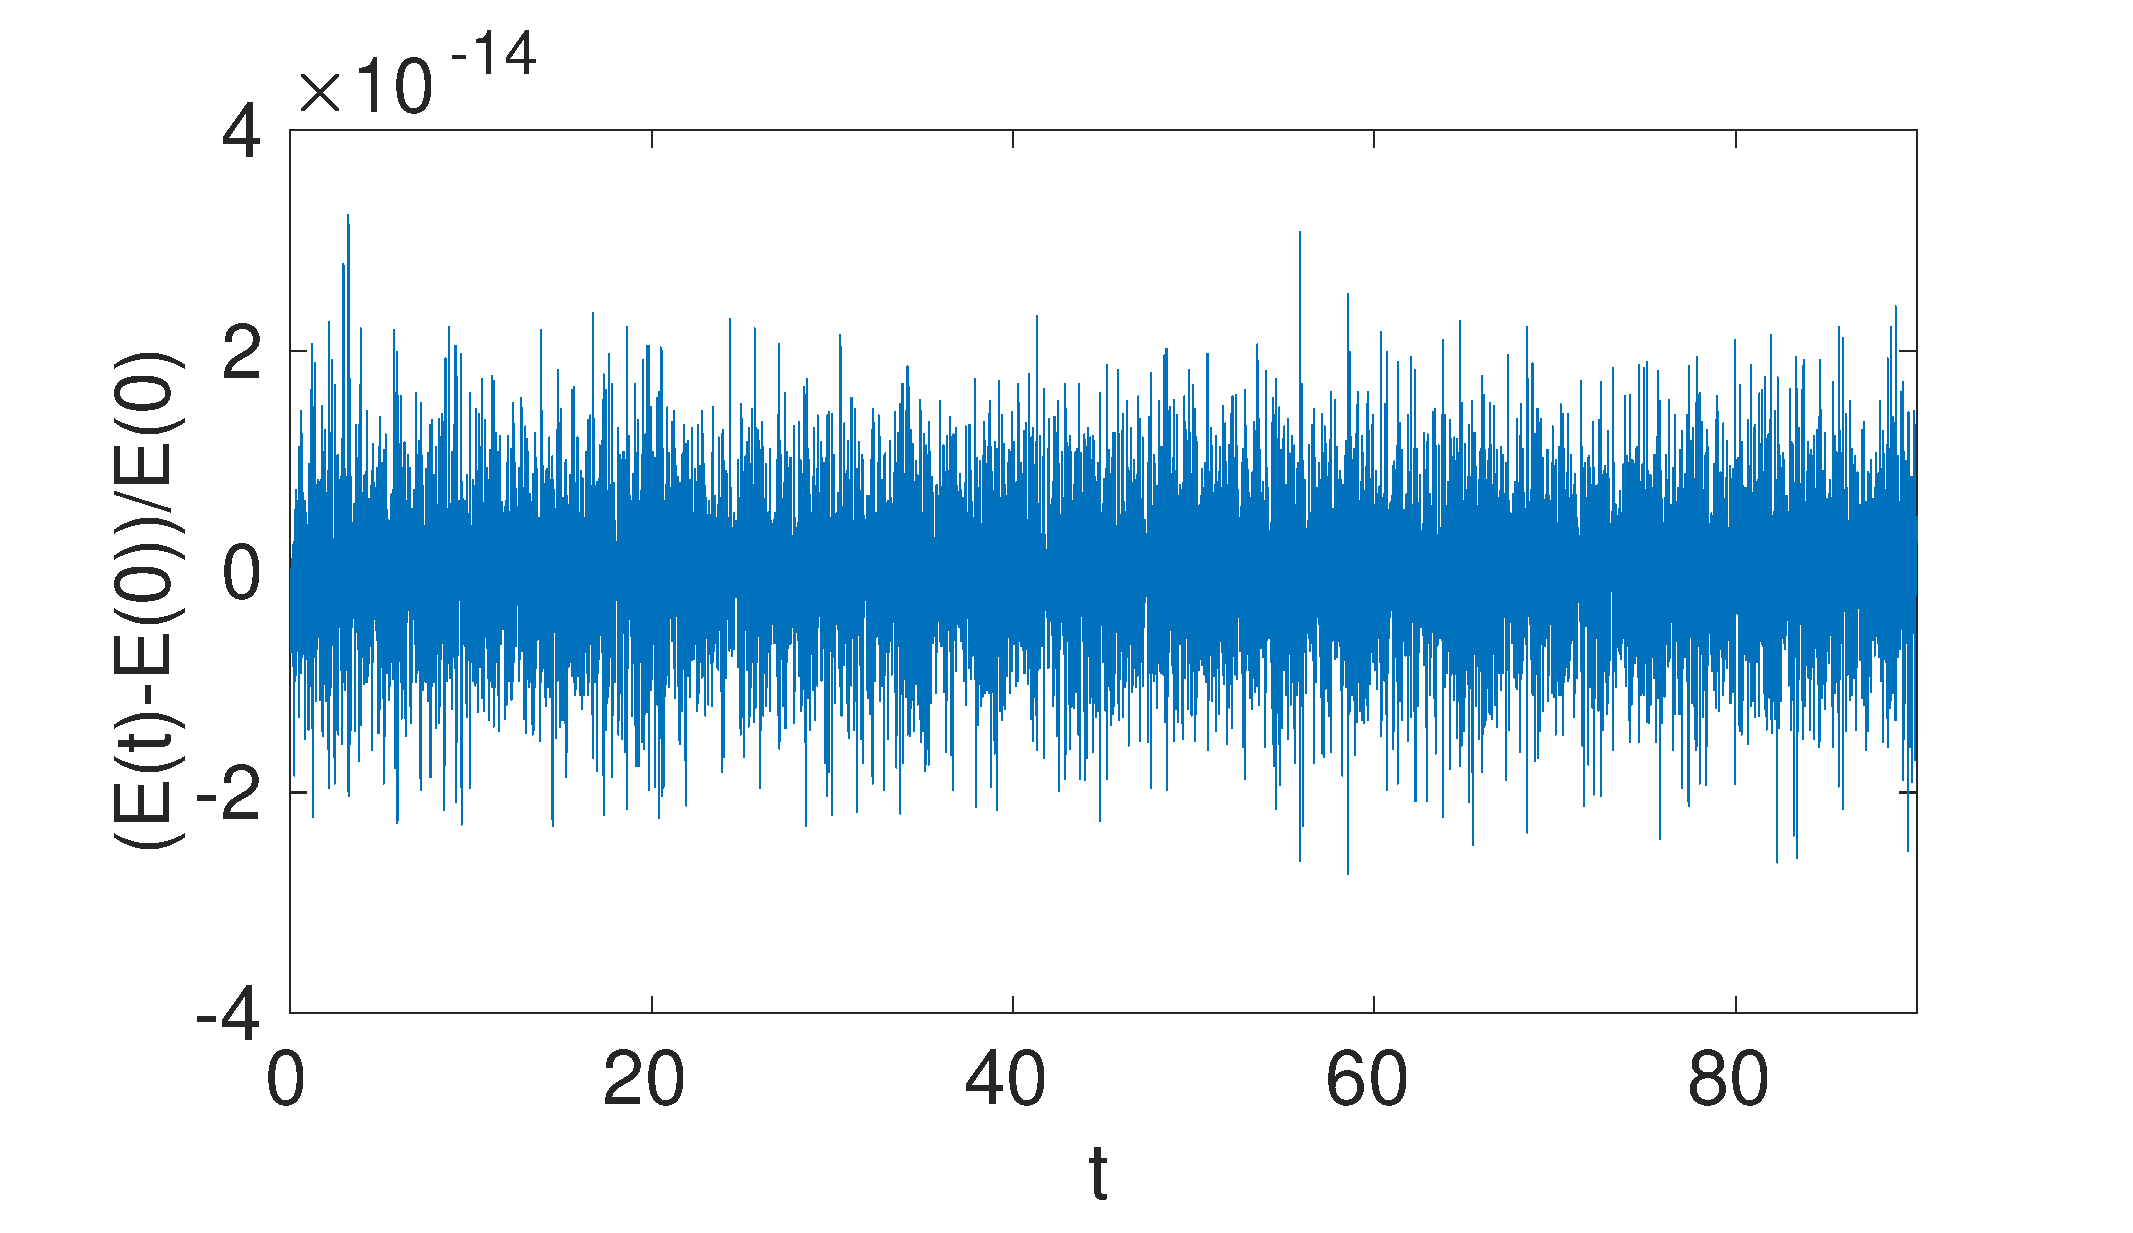
\includegraphics[width=0.6\textwidth,trim={0cm 0cm 0cm 0cm}, clip]{discrete_energy.eps}
	\caption{The relative change in fully discrete energy as a function of time. Here, $t = 90$ corresponds to $6186$ time steps}\label{discrete_energy}
\end{figure}




%!TEX root = elastic_3d_sbp.tex
\section{Conclusion}

\end{document}